\documentclass[manuscript]{aastex}

%-- Packages 
\usepackage[backref, breaklinks, colorlinks, citecolor=blue, linkcolor=magenta]{hyperref}

%\documentclass[]{emulateapj}
\newcommand{\vdag}{(v)^\dagger}
\newcommand{\myemail}{n.nicole.sanchez@vanderbilt.edu}

\slugcomment{Submitted to The Astrophysical Journal}

\shorttitle{Gas Accretion in MW-like Galaxies}
\shortauthors{N. N. Sanchez, J. M. Bellovary, \& K. Holley-Bockelmann}

\usepackage{natbib}
%\bibliographystyle{plain}
\bibliographystyle{apj}

\begin{document} 

\title{Cosmological Hydrodynamic Simulations of Preferential Accretion in the SMBH of Milky Way Size Galaxies}
%\title{A Particular Appetite: Cosmological Hydrodynamic Simulations of Preferential Accretion in the Supermassive Black Holes of Milky Way Size Galaxies}



\author{N. Nicole Sanchez \altaffilmark{1, 2}}
\author{Jillian M. Bellovary\altaffilmark{1, 2, 3}}
\author{Kelly Holley-Bockelmann\altaffilmark{1, 2}}

\affil{$^1$Fisk University, Nashville, TN, USA, n.nicole.sanchez@vanderbilt.edu}
\affil{$^2$Vanderbilt University, Nashville, TN, USA}
\affil{$^3$American Museum of Natural History, New York, NY, USA}


\begin{abstract}\label{abs:abstractlabel}

Using cosmological hydrodynamic simulations of Milky Way-type Galaxies, we explore the effect of accreted gas as feeding mechanisms for supermassive black holes. We examine two of these galaxies with differing merger histories using the Gasoline N-body+SPH code. One of there galaxies is characterized by several major mergers and the other with a quiescent history. We attempt to identify the importance of merger history on black hole accretion. Additionally, we consider a second, higher resolution version of the Milky Way-type galaxy with an active merger history using the Charm N-body GrAvity solver, ChaNGa.  This study is an extension of Bellovary et. al. 2013, which analyzed the accretion of high mass, high redshift galaxies and their central black holes. Bellovary found that the gas accreted by the central black holes was proportional to that accreted by the host galaxy. Contrary to the previous study's results, we've found that while a galaxy with a quiescent history will still have a SMBH whose accretion mirrors that of its host, a galaxy with an active merger history has a central black hole that is preferentially fueled by gas accreted through mergers. Through an investigation of the angular momentum of the gas entering these hosts and their SMBHs, we determine that merger gas enters the galaxy with lower angular momentum compared to smooth accretion, accounting for the preferential fueling witnessed in the SMBH of the galaxy with an active merger history. Our results imply that galaxy mergers play an important role in the feeding of the SMBHs in the class of Milky Way-type galaxies.

\end{abstract}

\keywords{Black hole physics -- Galaxies: spiral -- Galaxies: kinematics and dynamics -- Methods: Numerical -- Others?}

\section{Introduction}\label{sec-intro}

%[Note to self: Cite one canonical person but also more junior people in the field.]

%\citep[for example; ][at the end of the line]{Bellovary2010,Tremmel2015,Fu2008}
 %\S\ref{sec-intro}

Supermassive black holes (SMBHs) are thought to exist in almost all massive galaxies. \citep{Kormendy2013} In the canonical picture of BH growth, these black holes may become active galactic nuclei (AGN) during periods of high accretion and wane in periods of quiescence. \citep{Alexander2005,Papovich2006,Volonteri2012} The host galaxy's size, star formation rate, and other environmental effects may help to influence the growth of the black hole residing at its center; however, there are still uncertainties concerning the relationship between these SMBHs and their much larger host galaxies, as well as how they grow and evolve together. \citep[5-8 citations here]{Haehnelt2000,DiMatteo2005,Hopkins2006,Fu2008,Sijacki2009,Silverman2009,Mullaney2012}

The M$-\sigma$ relation, which relates the SMBH's mass and the velocity dispersion of the host galaxy's central stellar population, gives some insight into the complex interplay between these objects. \citep{Ferrarese2000} A prominent trend appears, as SMBHs tend to scale with the velocity dispersion of the host galaxy bulge. % For my thesis: A prominent trend appears as SMBHs tend to scale with the spheroidal center of their host galaxies; i.e. less massive SMBH reside in galaxies with less disperse bulges, and more massive SMBH live in galaxies with larger velocity dispersions in their bulges. 
The tightness of the relation is significant and can be seen over several orders of magnitudes in velocity dispersion and black hole mass. \citep{Merritt2001,Graham2011,Mcconnell2013,Kormendy2013} Scatter exists among the low mass galaxies and a deviation may appear at the high mass end, where overmassive BHs may reside. \citep{VanDenBosch2007,Moster2010,Natarajan2011} However, scatter in less massive galaxies may imply that there are several channels of black hole growth at play in the low mass end of the relation. \citep{Micic2007,Volonteri2009,Reines2013,Graham2014} One standard explanation for the M$-\sigma$ relation lies in galaxy mergers, which build up galaxies, feed SMBHs, and assemble bulges. \citep{DiMatteo2005,Shen2008} Major mergers are thought to supply gas to the central SMBH resutling in feedback which quenches star formation and affects the structure of the galaxy. 

% Kelly cut: In addition to the M$-\sigma$, other relations between the SMBH and its host have been well studied, making it clear that, though these objects have many orders of magnitude between their sizes, a complex interplay still exists.

%[CITE FOR THEORY: Springel and Dimatteo; cite when we discuss why m-sigma happens]
%McConnell and Ma have the prettiest M-sigma relation, but there are two camps: Kormendy and Ferrarese & Merritt who must both be cited.
%Check with Kelly: Which Van den Bosch, Emsellem, and Prija papers she would recommend.

% For thesis: M-sigma plot:
%\begin{figure}
%\centerline{\resizebox{0.75\hsize}{!}{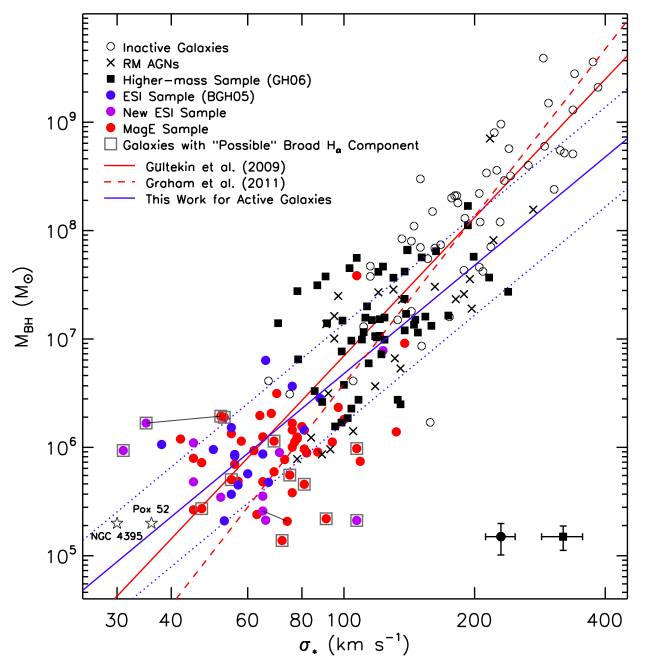
\includegraphics[angle=0]{fancymsigma}}}
%\caption[]{Gas fraction across redshift for galaxy (solid lines) and central BH (dashed lines). Green lines signify gas fractions accreted via mergers and blue lines designate gas accreted via cold flow.}
%\label{msigma} 
%\end{figure}
% Cite: Xiao

% For thesis: Explain feedback:
%Black hole feedback: the reaction effect of the energy obtained through gas accretion, which affects the overarching structure of the host galaxy.

% FOR SHOCKS: The simulations I am studying are run with a new implementation of Gasoline, which models hydrodynamic processes like shocks very well by using a geometric density average in the SPH force expression

The black hole mass-bulge luminosity relation was first implied by the work of \cite{Dressler1988}. \cite{Dressler1989} first proposed the correlation and it was first illustrated by \cite{Kormendy1993}. 
%The M$_{\rm BH}$-bulge mass relation followed and was determined via ground based observations by \cite{Magorrian1998} and was around M$_{\rm BH}$ $\sim$0.005 M$_{\rm bulge}$; however, this relation was characterized by a lot of scatter and its reliability waned due to selection biases.  
A wealth of evidence continues to relate these two characteristics, and follow up examinations using HST observations have determined the currect, best estimates yield a M$_{\rm BH}$/M$_{\rm bulge}$ fraction between about 0.0013 and 0.0023 \citep{Merritt2001a,McLure2001,Marconi2003}. 

Major mergers between massive galaxies are thought to be efficient fueling mechanisms for bright AGN. The large influx of material due to tidal torques from the merger causes bursts of star formation and helps funnel gas directly into the center where the SMBH resides. \citep{Richards2006,Reddy2008,Hopkins2010} Additionally, the most massive, highest-luminosity AGN (i.e. quasars) reside in incredibly luminous infrared galaxies where star formation is abundant, signifying that major mergers may have recently occurred. \citep{Treister2012} Distorted morphologies are often characteristics of quasar hosts, and companions can also be present around quasars, both of which are evidence that strengthen the possibility of a recent merger having affected their lifetimes. 

In many less massive and less luminous AGN, however, there is a clear lack of distorted morphologies, close neighbors, and/or other obvious merger evidence.  \citep{Ryan2007,Schawinski2011,Ellison2013,Hicks2013}[Maybe a different Ellison paper?] It is also important to note that many of these AGN exist in spiral galaxies, which are unlikely to have been recently disturbed by major mergers. \citep[Which 1990's Tremaine?]{Springel2005,Kocevski2011} Nevertheless, some evidence suggests \citep{vanGorkom1997,Governato2009} that disturbed galaxies may reform a disk quickly, even after a major merger as long as it is gas-rich. More recently, \cite{Treister2012} has suggested that only the highest luminosity AGN require fueling via major mergers; $\sim$90\% of AGN across all redshifts are fueled by various other mechanisms which may include minor mergers, flybys, and smooth accretion, whereby gas is directly accreted via large filaments from the ambient intergalactic medium \citep{Cox2006,Bellovary2013,Sinha2012}. 
Smooth accretion, in particular, may play an important role in fueling these low mass galaxies. Halos less than 10$^{11} M_{\odot}$ can accrete filaments of unshocked gas; thereafter, gas will shock heat to the virial temperature of the halo. \citep{Keres2005} Even for massive halos, unshocked gas may still penetrate shocked regions to fuel the galaxy. \citep{Brooks2007,Dekel2009,Nelson2013} Secular processes, including bar formation and disk instabilities, may also be prominent forms of accretion for these SMBHs. \citep{Kormendy2013}   

% For my thesis: The unshocked flow filaments that feed thses galaxies are dependent on the galaxy's mass. Smoothly accreted gas will fuel through unshocked gas filaments until the galaxy halo reaches a a mass near 10$^{11} M_{\odot}$. Once the galaxy's mass is greater than this threshold, the mass will reach the virial radius of the halo and the rapid increase in temperature within the radius causes the gas to shock as its temperature quickly increases.
	
It is clear that galaxy hosts grow through variety of channels that depend on mass, environment, and interaction history. Therefore, we want to understand how these different galaxy evolutionary paths translate into different SMBH fueling mechanisms, and see how they affect the fueling gas flowing into the SMBH itself. \cite{Bellovary2013} compared simulations of three high mass, high redshift galaxies and found that while mergers and smooth accretion both efficiently build up galaxies, no particular method was more adept at feeding the SMBH. Using a similar method as \cite{Bellovary2013}, this work compares the SMBH and galaxy fueling mechanisms between two Milky Way (MW) mass galaxies. 
	
We analyze two galaxy simulations that are similar at z = 0 but have very different merger histories. Our ``active'' galaxy, h258 \ref{h258face}, has a history characterized by major mergers, while our ``quiet'' galaxy, h277 \ref{h277face}, has a quiescent history with only minor mergers. Since these galaxies are similar to the MW in virial mass, stellar mass, and circular velocity, without a deeper examination, we may not recognize the varying histories that distinguish them. We will compare the origins of gas entering the SMBH and halo to look for clues about SMBH fueling within these galaxies. %Along these lines, we will also discuss the fueling mechanisms which vary between these galaxies of similar mass due to different merger and formation histories. 
MW-type galaxies host SMBHs on the order of 10$^6$ M, which are likely the most common type of massive black hole, yet little is known about them or how they may grow \citep{Kormendy2013}.  By examining the assembly of these galaxies, and their SMBH fueling, we compare the accretion rates between h258 and h277 to determine which accretion methods dominate in this class of galaxies.

%Note to self: Do I thoroughly discusses what we think we KNOW about growth/evolution and what is still being DEBATED?]	
  

% ##########################################################
% ##########################################################
% ########################################################## 
\section{Simulation Parameters}\label{sec-model}

[NOTE TO SELF: Make/include merger trees. Ask Christina?]

The cosmological simulations have been run using two smoothed particle hydrodynamics (SPH) N-body tree code: Gasoline \citep[][Stadel 2001, how do I cite a PhD thesis?]{Wadsley2004} and, more recently, Charm N-body GrAvity solver, ChaNGa. 

An initial DM-only, uniform resolution 50 comoving Mpc box determined which halos would be selected for zoom-in examination, including the two halos examined in this paper. The DM-only simulation assumed a WMAP Year 3 cosmology \citep{Spergel2007} with the following specifications: $\Omega _m$ = 0.24, $\Omega _{\Lambda}$ = 0.76, $H_0$ = 73 km/s, and $\sigma _8$ = 0.77. The halos h258 and h277  were chosen for their Milky Way-mass, between 6--8 $\times$ 10$^{11}$  M$_{\odot}$, at z=0 and their active and quiescent merger histories, respectively. The halos have virial masses defined relative to a critical density, $\rho _c$, where $\rho / \rho _c$ = 100 where h258 and h277 have virial masses of $M_{\rm vir} = 7 \times 10^{11} M_{\odot}$ and $M_{\rm vir} = 8 \times 10^{11} M_{\odot}$, respectively. A recent binary merger characterizes the h258 halo at z=1, while h277 has its last major merger near z $\sim$ 3. A second ``zoom-in'' high resolution simulation was run for both of these galaxies including gas and star particles using the volume renormalization of \cite{Katz1993}, resimulating only a few virial radii from the main halo at the highest resolution. Both simulations were run from z=150 to z=0.  [Make sure this is true for low res. True for high res.]

Gas can reach a minimum temperature of $\sim$100 K, without the inclusion of cooling via molecular hydrogen or metals. The simulation includes stochastically modeled star formation, including a star formation efficiency parameter of c$^*$ $=$ 0.1 and density threshold (2.5 amu cm$^{-3}$) for gas particles above which they become eligible to form stars; the gas must remain below a temperature threshold of 10$^4$ K. Star particles form along the Kroupa initial mass function \citep{Kroupa2001}. Supernova feedback releases $10^{51}$ ergs of thermal energy and affects a ``blastwave'' radius determined by the method of \cite{Ostriker1988}. In the affected region, cooling turns off for a time relative to the expansion phase of the SN remnant. SN Ia and II from \cite{Thielemann1986} and \cite{Woosley1986} are adopted, respectively, and implemented through the \cite{Raiteri1996} method. Both supernova ``blastwave'' radius calculations and supernova (Ia and II) prescriptions are as described in detail by \cite{Stinson2006}. A low-temperature extension to the cooling curve is used to trace metals \citep{Bromm2001}. Simulated galaxies are shown to conform with the observed Tully-Fisher relation \citep{Governato2009}, the size-luminosity relation \citep{Brooks2011}, and the mass-metallicity relation \citep{Brooks2007}, in addition to having realistic matter distributions and baryon fractions \citep{Governato2009a,Guedes2011}. These parameter and resolution choices allow the galaxies to adhere to the stellar-mass-halo-mass relation at z=0 and maintain a realistic period of star formation. \citep{Moster2010,Munshi2013,Brooks2007,Maiolino2008} We are confident with these criteria and restraints that we reasonably represent growth in the galaxy and its SMBH. We exclude AGN feedback in these small to moderate mass galaxies; however, we have determined that has little effect on the global properties of the galaxy and SMBH.
 
Since, there are uncertainties in the formation of black holes ``seeds,'' we implement a BH seeding method that is broadly consistent the theories of direct collapse black holes \citep{Couchman1986, Abel2002, Bromm2004} and Population III stellar remnants\citep{Loeb1994, Eisenstein1995, Koushiappas2004, Begelman2006, Lodato2006}. While this method allows the BH formation process to remain physically motivated. BH seeds form if their parent gas particle match the criteria required for star formation and also maintain zero metallicity. \citep{Stinson2006} A probability of $\chi_{\rm seed}$ ~ 0.01 is applied to determine whether a gas particle (with the above specifications) will become a BH seed with a mass of M$_{\rm BH}$ = 2.28 $\times$ 10$^5$ M$_{\odot}$, the same mass as its parent gas particle. This probability was chosen to match the predicted occupation probability of BH seeds at z $\sim$ 3. \citep{Volonteri2008} 
%This circumvents the Soltan argument wherein mergers alone are not the primary feeders of BHs, allowing for accretion growth to dominate \citep{Soltan1982}.  
BH seed formation ends at z $\sim$ 3.5 due to the dilution of pristine gas by efficient metal diffusion expected after the first population of supernovae. The requirement that BH seeds must form from zero metallicity gas particles also causes BH formation to be constrained in areas of early star formation bursts, where the earliest and most massive halos are expected to form in the simulation. BH formation is dependent only on their local environment, neglecting any large-scale properties of the host halo. Black holes are not fixed within the center of their host, allowing them to be dynamically affected by mergers and other perturbations within the galaxy. Nevertheless, BHs are kept near their host centers by choosing dark matter particles masses in high-resolution regions to be on the same order as gas particle masses which minimizes two-body interactions. \citep[Change citations?]{Bellovary2010,Zolotov2012}

Black hole mergers occur when they are separated by less than twice the softening length, and must be bound or satisfy $(1/2) \delta v^2 < \delta a \cdot \delta r$,  where $\delta v$ and $\delta a$ are the velocity and acceleration differences between the two black holes and $\delta r$ is the distance separating them. In addition to gaining mass via merger, black holes gain mass through Bondi-Hoyle gas accretion:
\begin{equation}
\dot{M} = \frac{4 \pi \alpha G^2 M^{2}_{\rm BH} \rho}{(c^{2}_{s} + v^2)^{3/2}},
\end{equation}
where $\alpha$ is a constant equal to 1, $\rho$ is the density of the surrounding gas, $c_s$ is the sound speed, and $v$ is the black hole's relative velocity to the gas. Feedback is applied to the surrounding gas as follows: $\dot{E}$ = $\epsilon _{r}$$\epsilon_{f}$$\dot{M}$$c^2$ where $\dot{M}$ is the accreted mass, and $\epsilon _r = 0.1$ and $\epsilon _f = 0.03$ are assumed for the radiative efficiency and feedback efficiency, respectively. This energy is distributed as thermal energy to the 32 nearest particles via a kernal probability function. Though other groups use a higher value for this efficiency, $\epsilon _f = 0.05$ \citep{Sijacki2007,DiMatteo2008} We find that $\epsilon_f = 0.03$ in our code produces MBHs in better agreement with MBH-host galaxy scaling relations. However, as our main concern is in the relative proportion of gas in various phases, our results are not sensitive to our choices of $\epsilon _{r}$ or $\epsilon_{f}$.
 
\subsection{Low Resolution GASOLINE Simulations}

Our low resolution simulations were first run using the smoothed particle hydrodynamics (SPH) N-body tree code Gasoline \citep[][Stadel 2001, how do I cite a thesis?]{Wadsley2004}, with a force resolution of 320 pc and the gas, dark matter, and star particle masses of 2 $\times$ 10$^5$ M$_{\odot}$, 3 $\times$ 10$^5$ M$_{\odot}$, and 7 $\times$ 10$^4$ M$_{\odot}$, respectively.  [Include starting numbers of gas, DM, and stars?] Both N-body+SPH volume renormalized simulations of h258 and h277 have been previously examined in other publications. \cite{Governato2009} studied the regrowth of the large disk structure in h258 by z=0 when such a recent merger affects the galaxy. This code includes a force resolution of 260 comoving pc, dark matter (DM) particles with masses of $1.3 \times 10^5 M_{\odot}$, and initial gas particle masses of $9 \times 10^4 M_{\odot}$.  

[NOTE TO SELF: Combine sub sections? This one is too short?]
	
%FOR THESIS ONLY: [Jillian's paper includes a table of simulation properties. Should I create one as well? I feel like yes.] 

\subsection{High Resolution CHANGA Simulations}

We used Charm N-body GrAvity solver, ChaNGa, a high resolution version of the same volume. The results of this paper, both from Gasoline and ChaNGa, utilize the same initial conditions but the latter is simulated at a higher resolution allowing the following new physics to be included: metal line cooling \citep{Christensen2012,Shen2010}, gas-phase and dust grain H$_2$ formation \citep{Christensen2014}, star formation dependence on H$_2$, and H$_2$ destruction from Lyman-Werner radiation. Other changes include a spline force softening lengths of 174 pc and initial gas particle masses of $2.7 \times 10^4 M_{\odot}$. Star particles are created with 30\% of their parent gas particle mass; therefore, a maximum initial mass of 8100 $M_{\odot}$. Each galaxy contains about 5 million DM particles inside the virial radius at z=0 and over 14 million DM, star, and gas particles total. The resolution of both force and mass in these simulations is comparable to the ``Eris'' simulation which has one of the highest resolutions for an N-body+SPH cosmological simulation of a Milky Way-mass galaxy so far produced.  At z=9, a uniform UV background is applied to simulate the cosmic reionization energy in a variation of \cite{Haardt2012}.

In this paper, we demonstrate that the results from this high resolution ChaNGa simulation has results which confirm those found by the low resolution Gasoline version of the same galaxy simulation. This secondary analysis allows us to feel confident in our results as we describe the varying origins of fueling gas accreting onto the simulated Milky Way-mass galaxy, h258.
	
%[Talk to Glenna about Ritchie Thomas forces]

% ##########################################################
% ##########################################################	
% ##########################################################
\section{Reduction Method}\label{redux}

	
The Amiga Halo Finder identifies all of the halos in the simulations by identifying the virial radii of the halos based on an overdensity using the criterion for a flat universe. \citep{Knebe2001,Knollmann2009,Gill2004} We select the primary halo by determining the most massive galaxy at z=0 and locating the central SMBH. For our Gasoline simulations, both the primary halo in h258 and h277 had final masses on the order of $10^{12} M_{\odot}$ and a formation redshift of z~4.  

EDIT: Include specs: mass, formation z, N (just for primary halos? Ask Kelly what she means.)

In this analysis, we trace gas particles from their origin through their journey into the galaxy and SMBH to determine their position within the SMBH or its host \citep{Brooks2009} . We then trace the SMBH back through time, determining its host halo in each snapshot. As we discussed in the introduction, there are a variety of fueling mechanisms thought to grow SMBH. Gas particles are initially traced prior to their accretion onto the main halo to determine whether they occupied a different halo at their formation. The particles are then classified by their method of entrance into the primary halo. If the gas particles existed in the primary halo at the first time step, they are classified as ``early'' gas. Gas that belonged to a different halo than the primary prior to accretion is classified as ``clumpy'' and enters the primary halo through mergers. All other gas is classified as entering the halo via ``smooth'' accretion, and is then subdivided into two categories: ``cold'' and ``shocked.'' In the cases where a shock does not develop, unshocked gas will usually flow into the halo via large-scale, dark matter filaments. (Bellovary 2013) It's possible for the filaments to also be dense enough to pierce an already developed shock allowing for unshocked gas to funnel into the galaxy core where it can accrete onto the SMBH without being heated to the virial temperature.
	
%[Kelly question: If the fingerprint of the fuel inflow is unique, can the angular momentum of the gas infer spin? Answer: no, can't infer spin from angmom of gas at 100 pc res.]

As previously described, if the galaxy halo is around or greater than 10$^{11}$ M$_{\odot} $, the gas will shock. We determine shocked particles through an increase in entropy and temperature using the following criteria:
\begin{equation}
T_{\rm shock} \geq 3/8 T_{vir}
\end{equation}
where T$_{\rm vir}$ is the virial temperature of the halo and T$_{\rm shock}$ is the temperature of the gas particle, and 
\begin{equation}
\Delta S \geq S_{\rm shock} - S_0
\end{equation}
where S$_0$ is the initial entropy of the gas particle and 
\begin{equation}
S_{\rm shock} = log_{10}[3/8 T_{\rm vir}^{1.5}/4 \rho_0]
\end{equation}
where $\rho_0$ is the gas density prior to experiencing the shock. The galaxies in this study reach final masses on the order of 10$^{12}$ M$_{\odot} $, therefore, shocked gas begins to enter the galaxy by the later timesteps of our simulation when it has reached this critical mass. 

% [REPEAT] Gas entering the halo via smooth accretion, whether unshocked or shocked, is traced to 0.1 R$_{vir}$ from the galaxy, a distance after which the thermal status of the particle can no longer be confidently tracked, as supernova feedback can mimic virial shocking. Gas particles that reach this distance with the above increased in entropy and density are considered shocked particles, while all others are categorized as unshocked. (``See Brooks et. al. 2009 for complete details about shock physics.'')\\

Once all the gas particles have been individually categorized, we can use these labels to determine the methods of accretion onto these Milky Way-size galaxies. With the information about which particles are accreting onto the SMBH (from the gas reservoir of particles that have been accreted by the galaxy), we can better compare the methods feeding both the galaxy and its SMBH. We can then determine whether there exists a method more efficiently building up these kinds of galaxies and their SMBH.

% ##########################################################
% ##########################################################
% ##########################################################
\section{Results} \label{results}

From the initial analysis of the low resolution Gasoline simulations, we have determined that the merger histories of these two galaxies has a pronounced effect on the resulting accretion of gas into the SMBH and its host. 

\subsection{Gasoline - Low Resolution h258: Resolution Test}
	
The galaxy, h258, is characterized by an active merger history including a major merger at z=1. The merger can be seen affecting the cumulative black hole mass (Figure \ref{h258allmassgas}) as well as the gas fractions within the both the SMBH and galaxy (Figure \ref{h258numfrac}). 
Figure \ref{h258allmassgas} shows h258's central SMBH's cumulative mass as a function of time (lower axis) and redshift (upper axis). The black dashed line indicates the total cumulative BH mass (including both mass from gas and BH mergers), while the black solid line indicates only the total gas mass accreted by the BH. The blue dot-dashed line indicates the gas mass accreted via unshocked gas. The green solid line indicates the gas mass accreted through mergers. The red dashed line indicates gas mass that was shocked upon entry into the halo. Though this figure shows that the primary source of mass gain at high redshifts is through mergers with other black holes, there is a significant increase in the amount of gas adding to the mass of the SMBH starting at z $\sim$ 1, where we know a major merger takes place. \textbf{[Reference merger tree here once you've added it.]} Figure \ref{h258numfrac} shows the fractions of unshocked and clumpy gas compared to all accreted gas as a function of redshift. It confirms that unshocked gas (blue) makes up the majority of gas entering the galaxy (solid lines) at early times; nevertheless, around the time of the merger (z $\sim$ 1) a marked change occurs in the gas fractions within the black hole (dashed lines) where clumpy gas (green) becomes the main component of total gas. 

Figure \ref{h258stackfrac} depicts the fractions of total gas in the galaxy (a) and the SMBH (b) at z=0, again differentiated by the gas particles' origins. Blue, green, and red distinguish cold, clumpy, and shocked, respectively. Yellow indicates gas that existed within the main halo upon formation. The galaxy has a mass nearly half comprised of gas entering the galaxy through unshocked, smooth accretion (48 \%), with 39 \% of the gas entering through mergers. The smallest fractions of the total gas are comprised of shocked gas (9 \%) and ``early''gas which existed at formation makes up the final, smallest fraction (4 \%). Unlike the galaxy, nearly 65 \% of the gas accreted by the central SMBH was gas accreted via mergers, while only a quarter (26 \%) is comprised of unshocked, smoothly accreted gas. Shocked gas makes up the last 9 \% of total gas entering the SMBH, along with a negligible ($<$ 1\%) amount of ``early'' gas. \textbf{So Figure \ref{h258stackfrac} shows explicitly that the SMBH more readily accretes gas gained through mergers.} This result is \textit{contrary} to the previous results of \cite{Bellovary2013} which found that the fractions of gas comprising the SMBH's total gas mass and that in its host were nearly the same. This result is surprising, but important, as it allows us to consider that a different physical mechanism characterizes the gas entering this MW-type galaxy than those affecting the gas accretion of the high mass galaxies examined by \cite{Bellovary2013}. 

We examine the angular momentum of the gas at the moment it enters the galaxy for clues to the understand the ready accretion of merger accreted gas. (Figure \ref{h258angmom}) A cumulative distribution of the angular momentum of entering gas, differentiated based on method of entrance into the galaxy, shows that gas entering the SMBH (dashed lines) has an overall lower angular momentum than gas entering galaxy (solid lines). This statement is true whether the gas enters via unshocked smooth accretion, becomes shocked upon entry, or enters through a galaxy merger (blue, red, green, respectively). Therefore, we can infer from this plot that lower angular momentum gas more readily flows into the central region of the host galaxy where it can be accreted by the black hole. In contrast, \cite{Bellovary2013} found a \textit{slight} preference for gas of a lower angular momentum to enter the SMBH. The question remains, however, as to why unshocked gas contains some of the lowest angular momentum gas while clumpy gas nevertheless appears most prominently in the SMBH at z = 0. The answer to this conundrum may lie in the major merger that characterizes this galaxy, so we look specifically at the gas accreted during the merger. 

Figure \ref{h258angmom_merger} explicitly shows that at the time of the merger, clumpy gas (green) has the lowest angular momentum entering the galaxy (solid lines) or the SMBH (dashed lines). Both cold gas and shocked gas (blue and red, respectively) are entering the galaxy and SMBH with significantly higher angular momentum. Therefore, as we've already seen that the SMBH tends to preferentially accrete gas with lower angular momentum, we determine that the significantly lower angular momentum with which the clumpy gas enters the galaxy at this timestep, allows for nearly all of the clumpy gas to then funnel directly into the SMBH. It is clear through this result the physical properties afecting the galaxy through this major merger play an important role in allowing for the direct fueling of the SMBH at its center.

\textit{NOTE: Need to add a figure that clearly supports this argument. Possibly a series of angular momentum plots at the times of mergers. Or comparisons between cumulative distributions at time with and without mergers.}

\subsection{Gasoline - Low Resolution h277: Resolution Test}
	
Our quiescent galaxy, h277, was characterized by few mergers in its past, its final major merger occuring around z $\sim$ 3. This merger is visible in Figure \ref{h277allmassgas}, though more subtle than the influx of gas in h258. (Linestyles as in Figure \ref{h258allmassgas}.) In h277, gas seemed to be gained at a more steady rate and at fairly high redshifts comprises a larger portion of the BH's total mass than seen in the previous, more active galaxy. The gas fractions (Figure \ref{h277numfrac}) in h277 (solid lines) and SMBH (dashed lines) are also markedly different than that of a galaxy with an active merger history. While it appears neither clumpy or unshocked gas (green and blue, respectively) particularly dominates at higher redshifts in the galaxy, merger gas becomes prominent in the SMBH at times when mergers occur. \textbf{[Ref merger tree when included.]} Again, this implies some physical process allowing merger gas to readily fuel black hole growth. Though, it is important to note that by z $\sim$ 0, smoothly accreted, unshocked gas again dominates in both the SMBH and host galaxy. As in our more active galaxy, it appears that the role of clumpy gas as it fuels the SMBH becomes important when mergers affect the galaxy; however, with h277 having a significantly less active merger history, unshocked, smooth accretion inevitably dominates the total gas supply.

This result can be more clearly seen in Figure \ref{h277stackfrac}. (Colors as in \ref{h258stackfrac}.) Similar to Bellovary et. al. 2013 study, which found SMBH accretion in high mass, high redshift galaxies mirror their hosts in terms of accreted gas, h277's SMBH accretes a similar fraction of each type of gas, comparable to its host galaxy. Smoothly accreted, unshocked gas represents about half of the total gas in both the SMBH and the galaxy. Clumpy gas also maintains about 30\% of both, while an increase in shocked gas occurs, from 13 \% in the galaxy to 22 \% in the SMBH. %; however, we argue this may be due to supernova contamination in the simulation. 
So by present day, h277 found no strong preference for the SMBH to prefer any one kind of gas in its accretion. Like the SMBHs in the study of \cite{Bellovary2013}, nearly the same fractions of gas entering the halo would then be accreted onto the SMBH (with the exception of shocked gas). Therefore, this may imply that without some physical driver, like the major merger of h258, clumpy gas is unlikely to dominate the gas accreted into the SMBH.

As in the previous case, we examined the angular momentum of all the gas particles accreted by the SMBH and host galaxy at the moment of entry. (Figure \ref{h277angmom}; Linestyles as in \ref{h258angmom}) Like before, it is immediately apparent that the clumpy gas accreted by both the black hole and its host has a lower angular momentum overall than the smoothly accreted gas; however, unlike we found in h258, the h277 galaxy accretes gas with lower angular momentum than that of its SMBH. This appears to imply that some of the gas with the lowest angular momentum is remaining in the host galaxy rather than accreting onto the SMBH. 

% IS THIS WHAT IT MEANS? This means that even though some of the gas in the host halo had lower angular momentum, that gas didn't find its way into the central region to accrete onto the BH. This may again imply that some physical phenomena is required to drive those gases towards the center. 

As h277 and h258 are similar in size and appearance at z=0, these differences indicate that the varying histories of these simulations appears to play an important role in the evolution of these types of galaxies and their central SMBHs. We also note that while mergers may not be the only physical mechanisms by which gas can be funneled into the centers of galaxies, mergers between galaxies clearly play an important role when considering the gas accretion of SMBHs.

\subsection{ChaNGa - High Resolution h258}

Just as we found in the lower resolution simulation, the high resolution sees a distinct preference for accreting gas that has been gained through the many mergers in its history. 


\section{Conclusion}

[Still need to write; Yes still need to write]


\acknowledgments
Thank you to the Fisk-Vanderbilt Masters-to-PhD Bridge program for their continued funding and support. [GET GRANT NUMBER]

%\begin{figure}
%\centerline{
 % \resizebox{0.95\hsize}{!}{\includegraphics[angle=0]{fig1a.pdf}}
  %}
%\centerline{
 % \resizebox{0.95\hsize}{!}{\includegraphics[angle=0]{fig1b.pdf}}
  %}  
  %\centerline{
  %\resizebox{0.95\hsize}{!}{\includegraphics[angle=0]{fig1c.pdf}}
  %}
%\caption[]{Evolution of our flat rotating model (A0) in isolation.
%Top Panel: Stellar density profile at various times. $\gamma = 1.0$ is the reference theoretical profile, shown as a dashed line. Middle Panel: Evolution of intermediate to major (b/a) and minor to major %(c/a) axis ratio as measured at the half mass radius. Bottom Panel: Ratio of rotational velocity to the 3-d velocity dispersion as a function of distance at various times. In isolation, the rotational support in the center decreases over time as the central SMBH increases the velocity dispersion.
%} \label{stab}
%\end{figure} 

\begin{figure}
\centerline{\resizebox{0.75\hsize}{!}{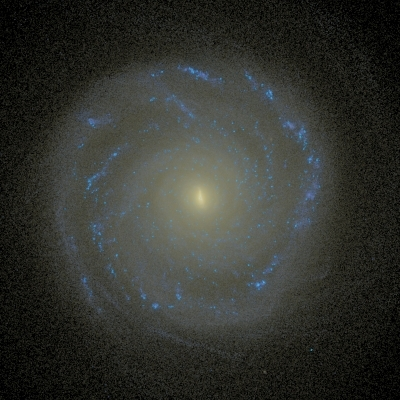
\includegraphics[angle=0]{h258_faceon_crop}}}
\caption[]{Face-on and edge-on Sunrise images of our GASOLINE galaxy, h258, which has an active, merger-rich history.}
\label{h258face} 
\end{figure}

\begin{figure}
\centerline{\resizebox{0.75\hsize}{!}{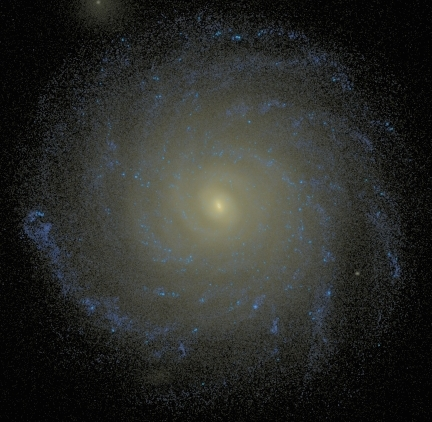
\includegraphics[angle=0]{h277_faceon}}}
\caption[]{Face-on and edge-on Sunrise images of our GASOLINE galaxy, h277, which has a quiescent, merger-quiet history.}
\label{h277face} 
\end{figure}

\begin{figure}
\centerline{\resizebox{0.75\hsize}{!}{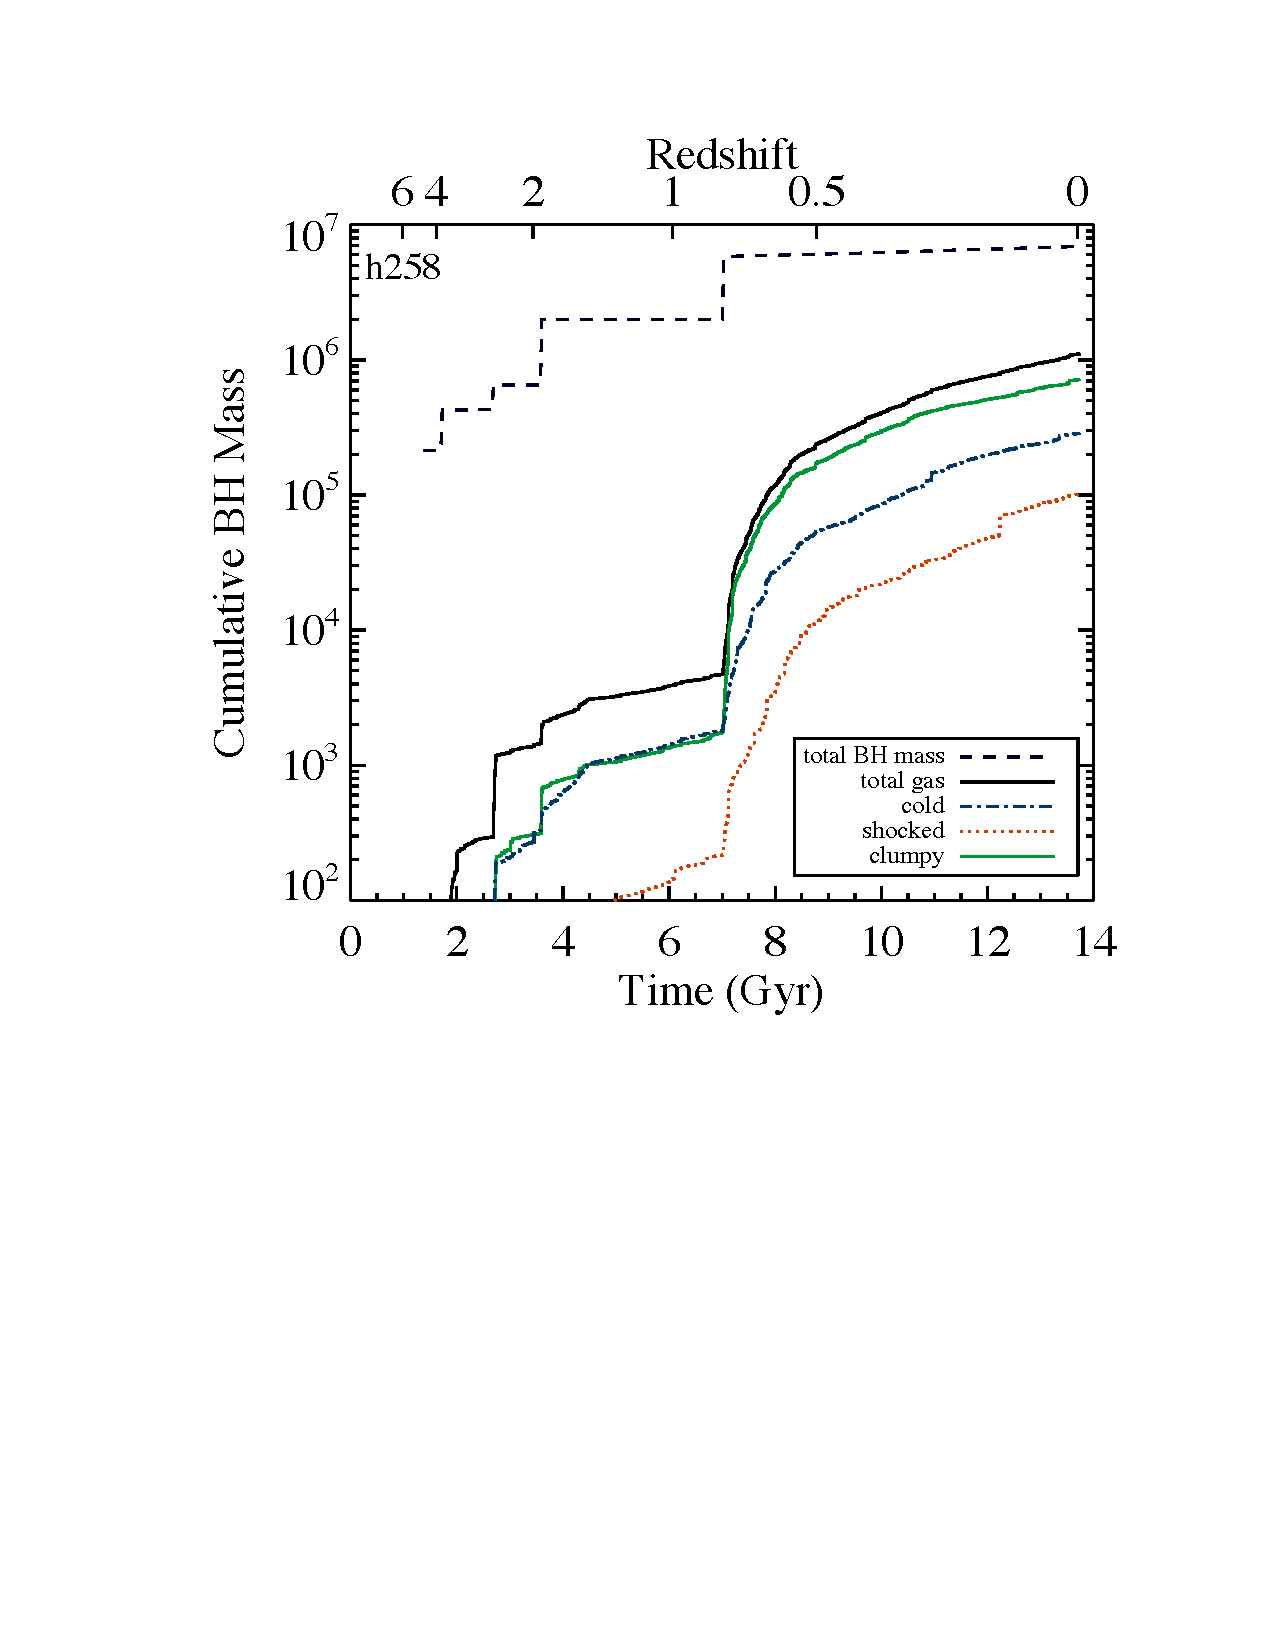
\includegraphics[angle=0]{h258_allmassgas_final}}}
\caption[]{The central BH’s cumulative mass as a function of time and redshift. The black dashed line indicates the total cumulative BH mass. The black solid line indicates the total gas mass. The blue dot-dashed line indicates the gas mass accreted via unshocked gas. The green solid line indicates the gas mass accreted through mergers. The red dashed line indicates gas mass that was shocked upon entry into the halo.}
\label{h258allmassgas} 
\end{figure}

\begin{figure}
\centerline{\resizebox{0.75\hsize}{!}{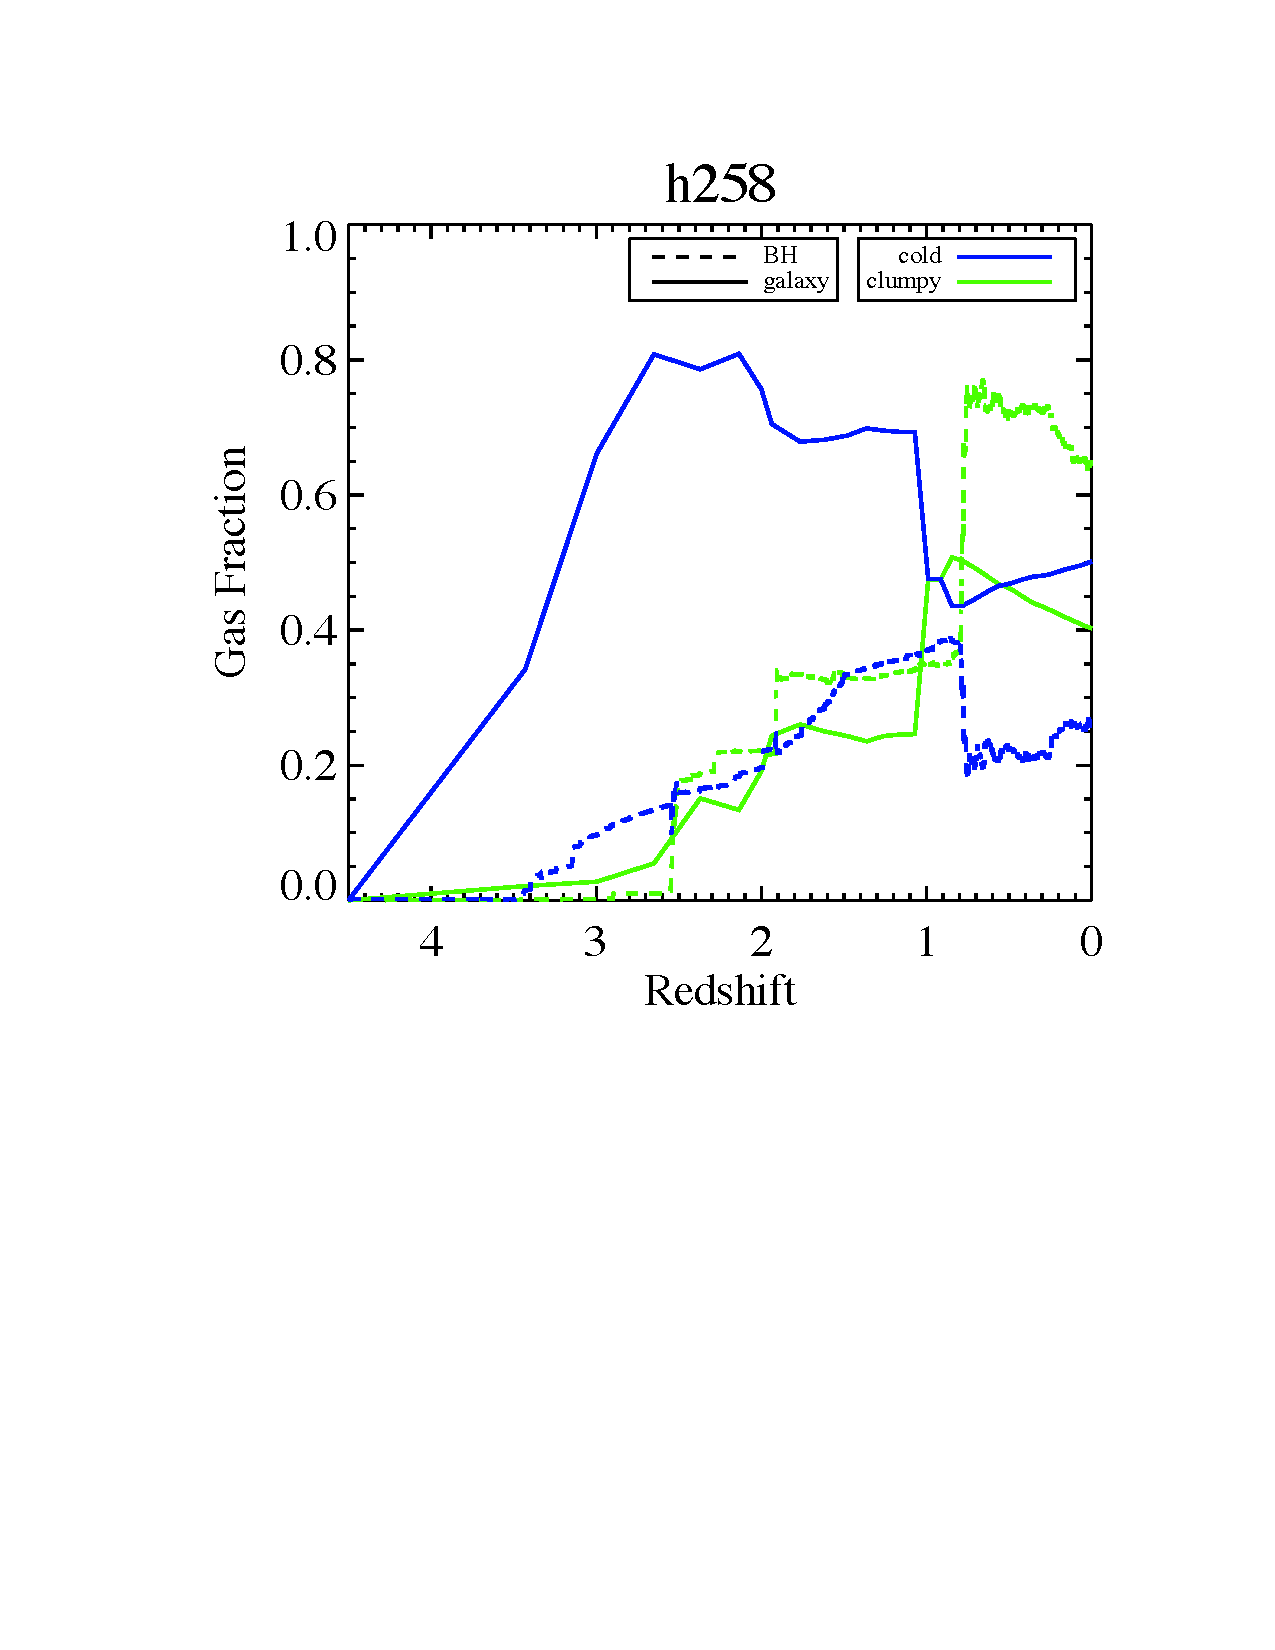
\includegraphics[angle=0]{h258numfraction_brightgreen}}}
\caption[]{Gas fraction across redshift for galaxy (solid lines) and central BH (dashed lines). Green lines signify gas fractions accreted via mergers and blue lines designate gas accreted via unshocked gas filaments.}
\label{h258numfrac} 
\end{figure}

\begin{figure}
\centerline{\resizebox{0.75\hsize}{!}{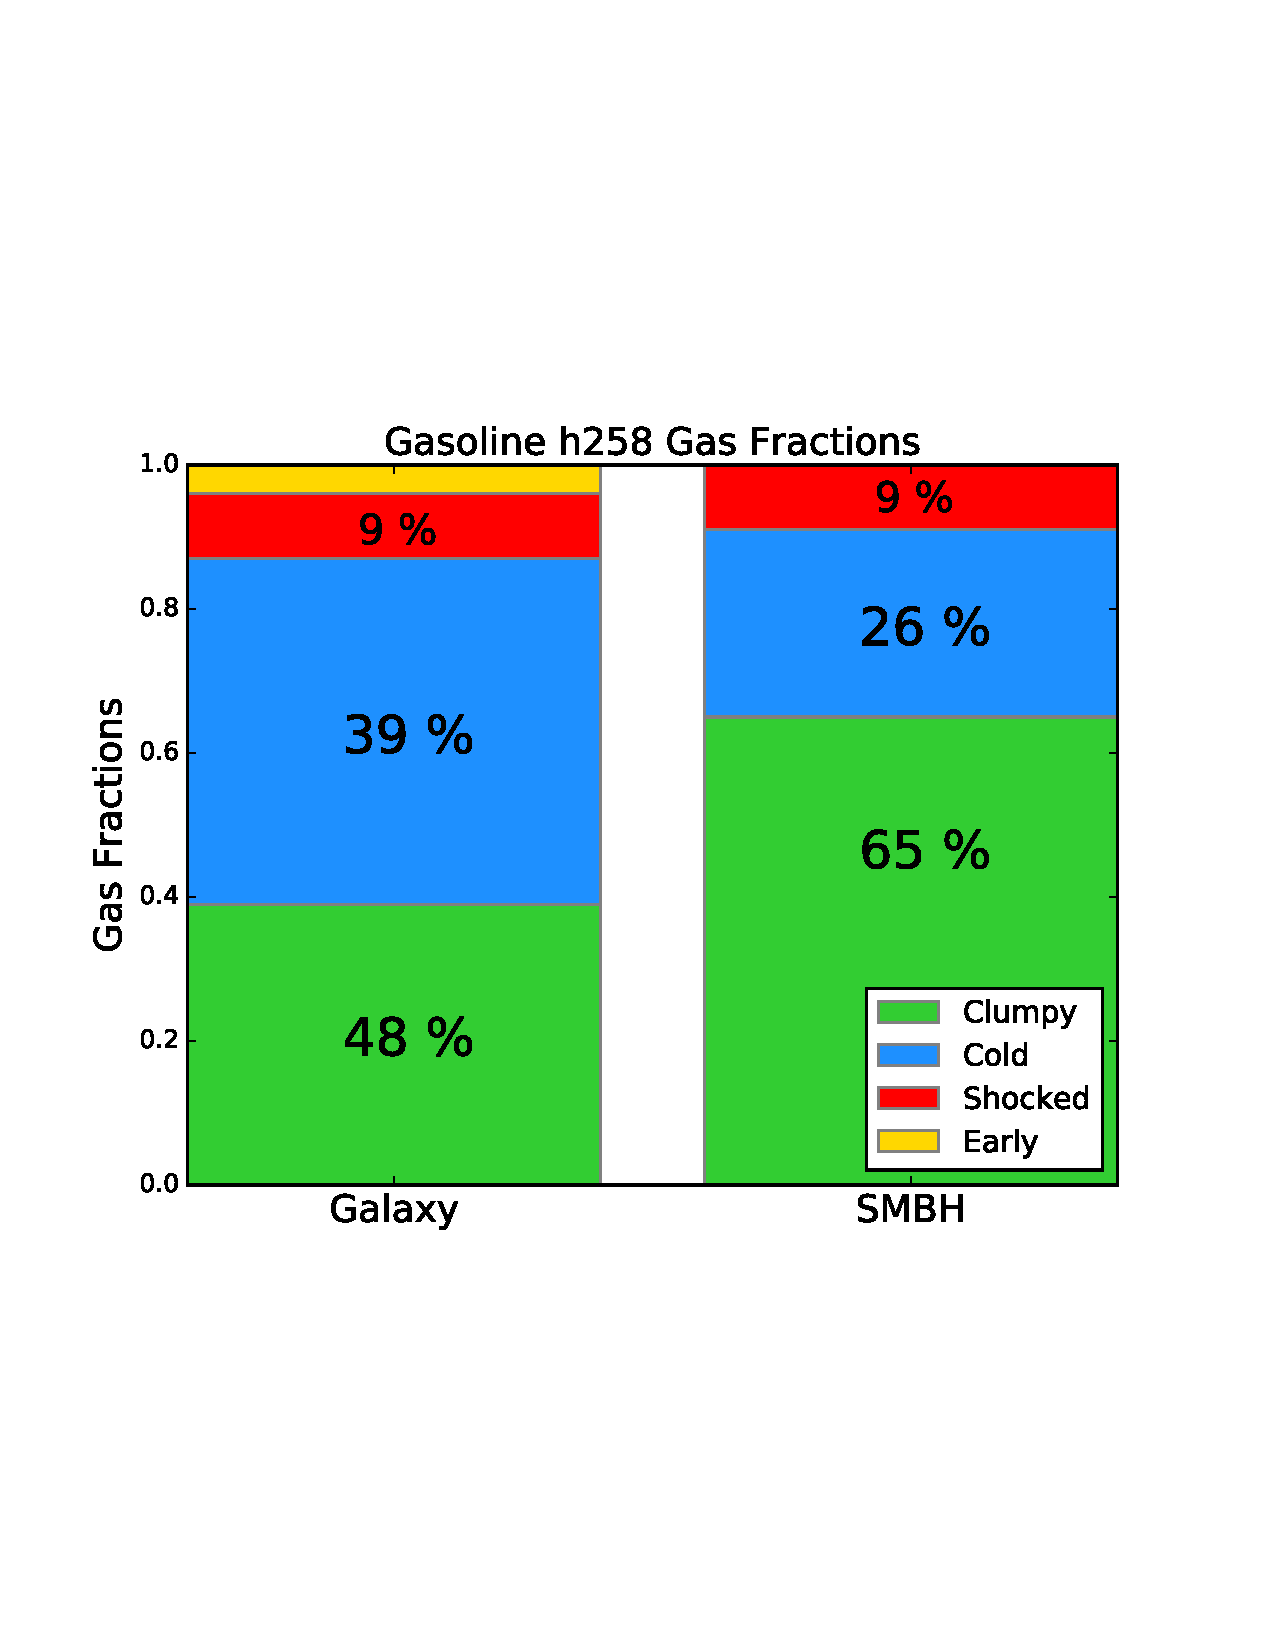
\includegraphics[angle=0]{h258_stackbarfractions}}}
\caption[]{Gas fractions of the gas particles accreted in h258 by the main halo (left) and the SMBH (right), distinguished by type. Blue, green, and red distinguish gas gained through unshocked gas, gained through mergers, and gas shocked upon entry, respectively. Yellow indicates gas that existed within the main halo upon formation; this ``early'' gas is negligible ($<$ 1 $\%$) within the SMBH.}
\label{h258stackfrac} 
\end{figure}

\begin{figure}
\centerline{\resizebox{0.75\hsize}{!}{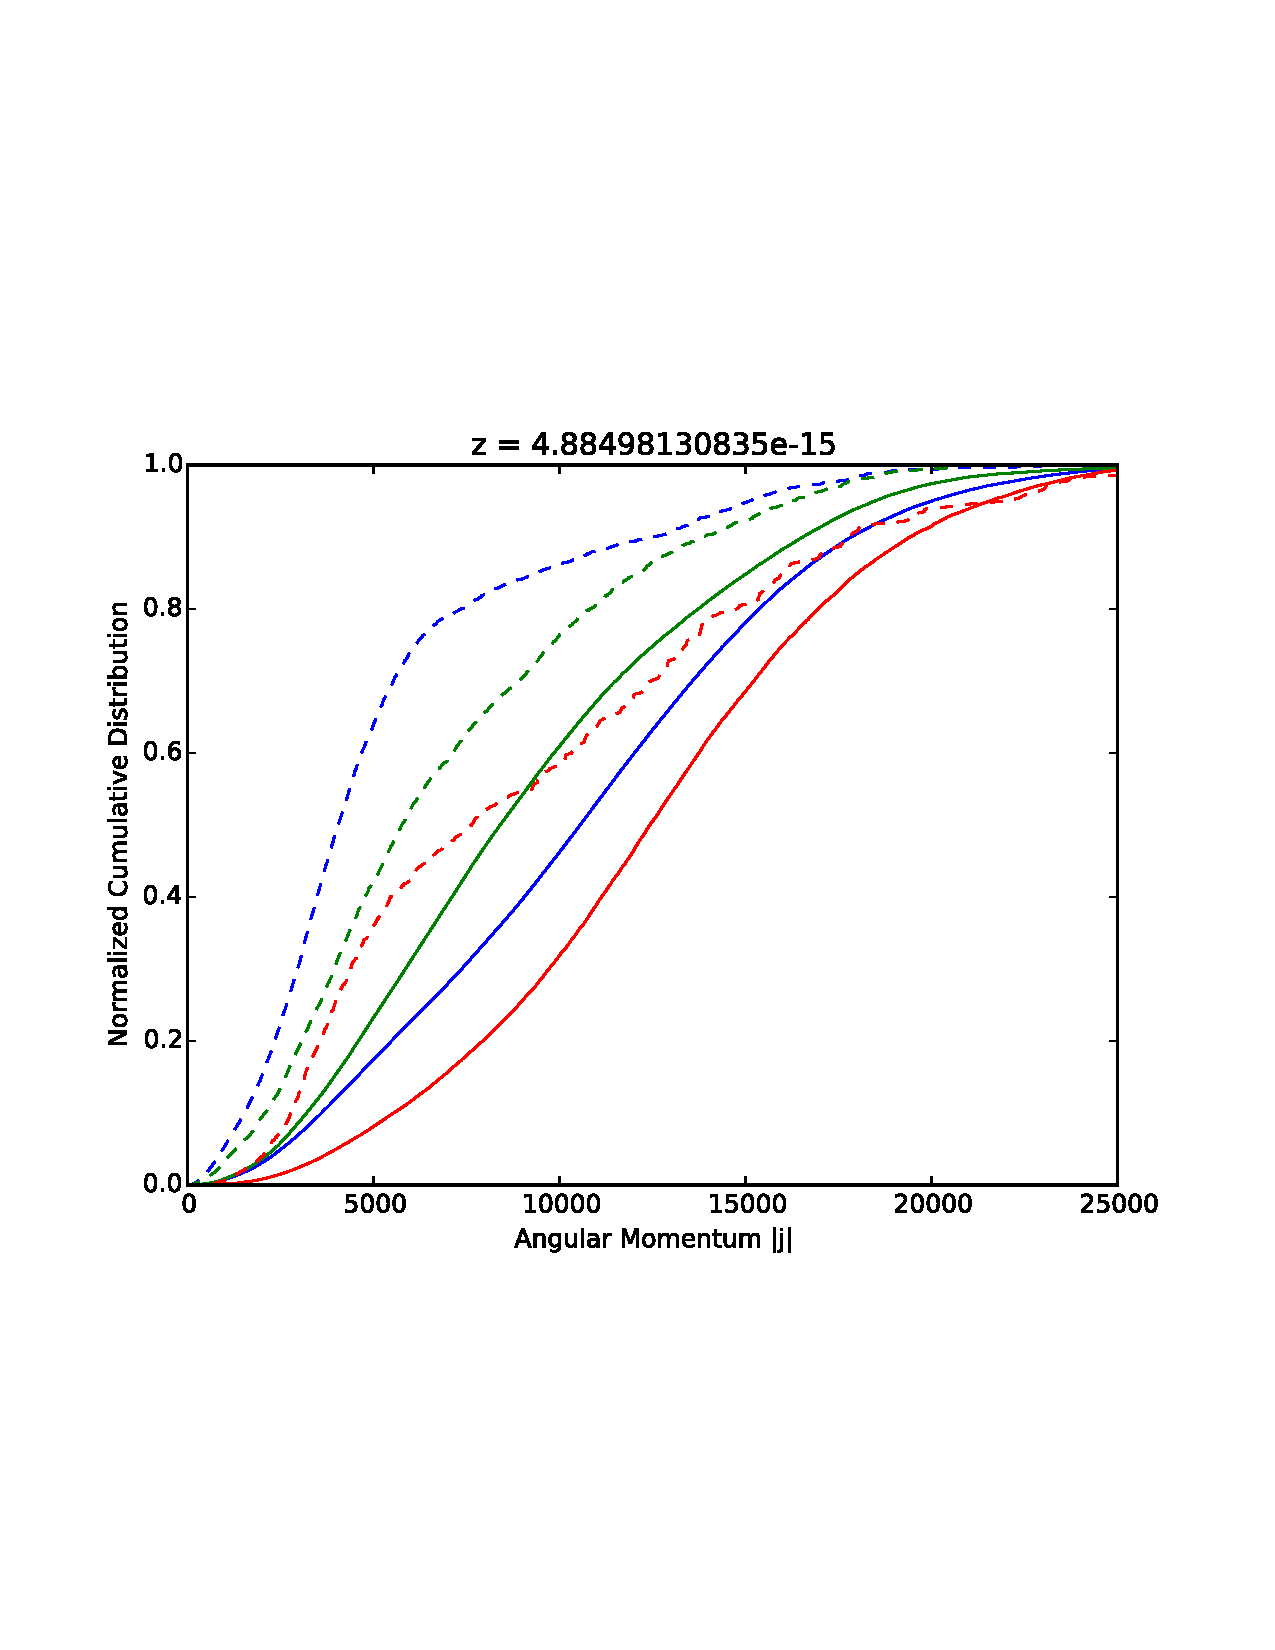
\includegraphics[angle=0]{h258_angmom_cumudist}}}
\caption[]{ Cumulative distribution of angular momentum of the gas particles accreted onto h258.  Gas particles accreted onto the main halo (solid lines) and central black hole (dashed lines). The green, blue, and red lines indicate clumpy, unshocked, and shocked gas, respectively.}
\label{h258angmom} 
\end{figure}

\begin{figure}
\centerline{\resizebox{0.75\hsize}{!}{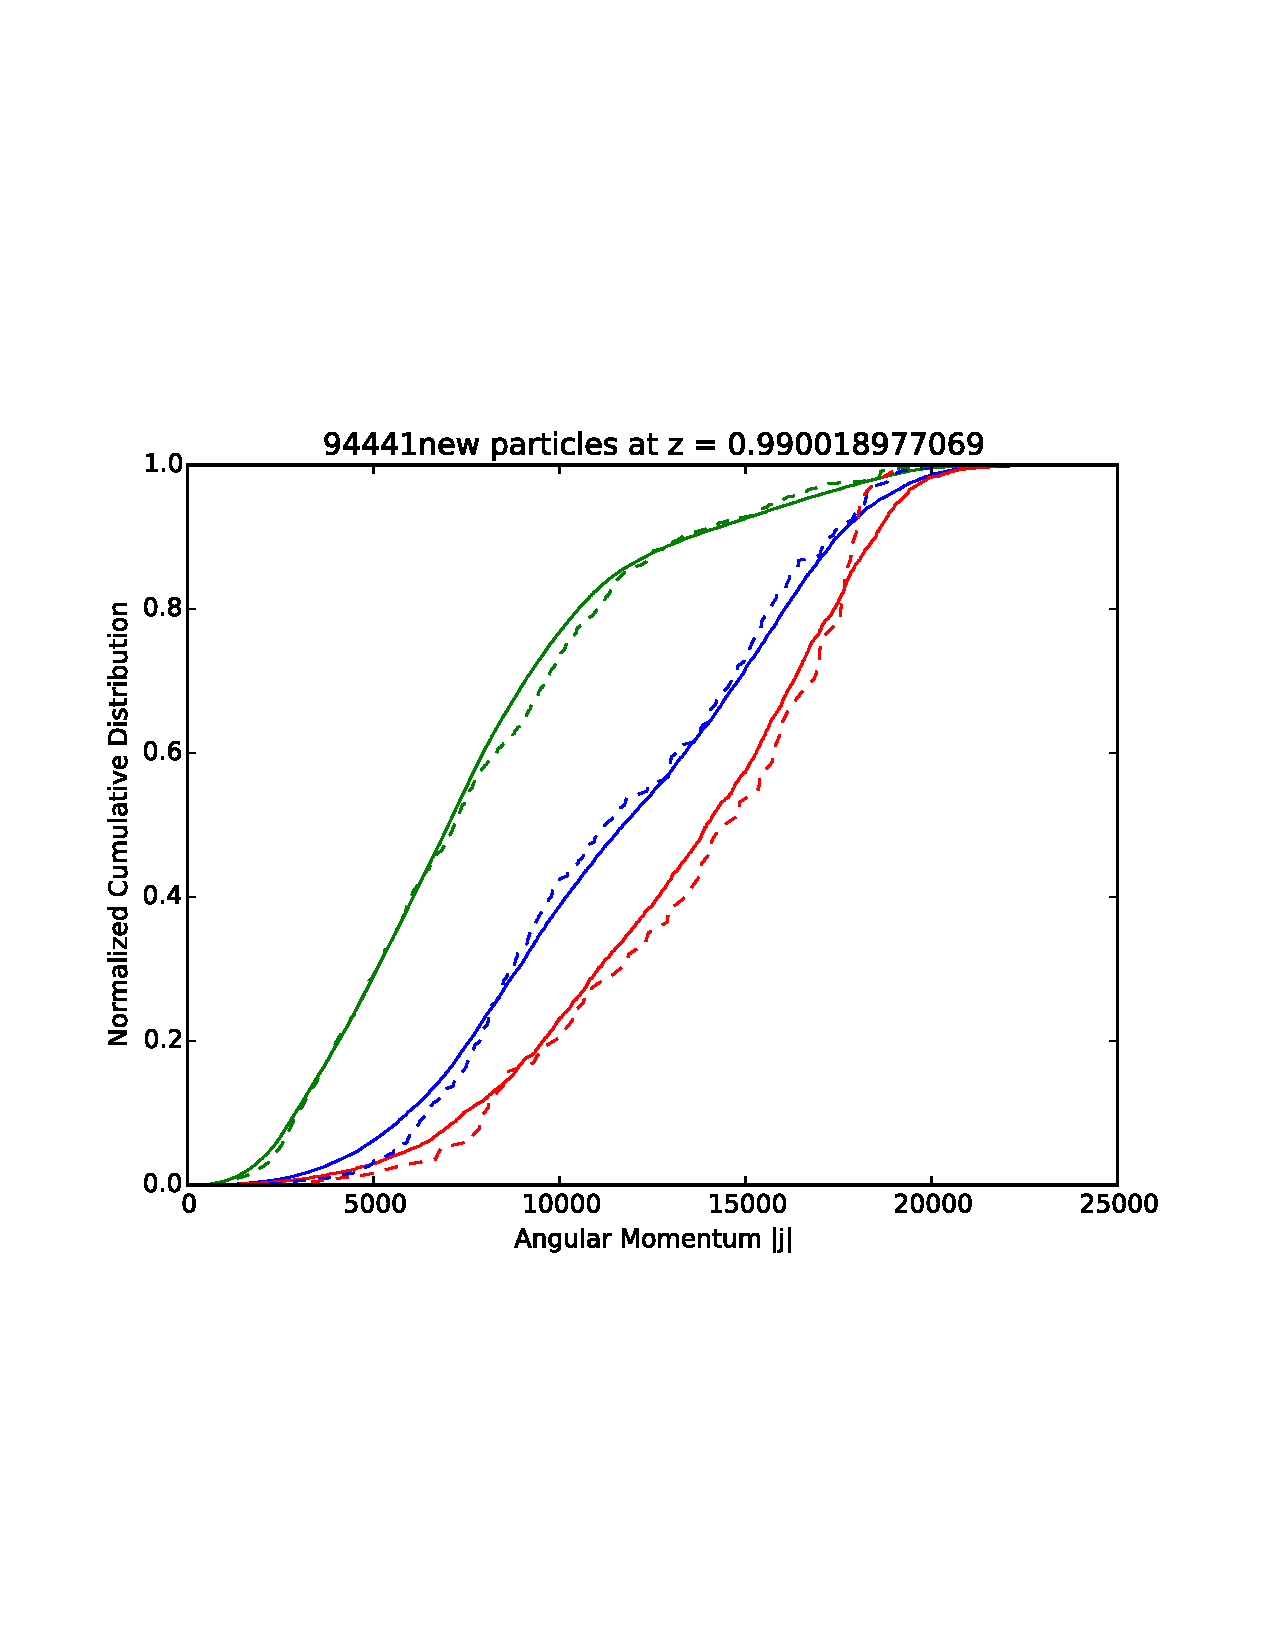
\includegraphics[angle=0]{h258_am_tsnew_228}}}
\caption[]{ Cumulative distribution of angular momentum of the gas particles accreted onto h258 at the time of the major merger (z ~ 1). There are about 95,000 gas particles accreted at this timestep, which gas particles accreted onto the main halo and central black hole distinguished by solid and dashed lines. The green, blue, and red lines indicate clumpy, unshocked, and shocked gas, respectively.}
\label{h258angmom_merger} 
\end{figure}

\begin{figure}
\centerline{\resizebox{0.75\hsize}{!}{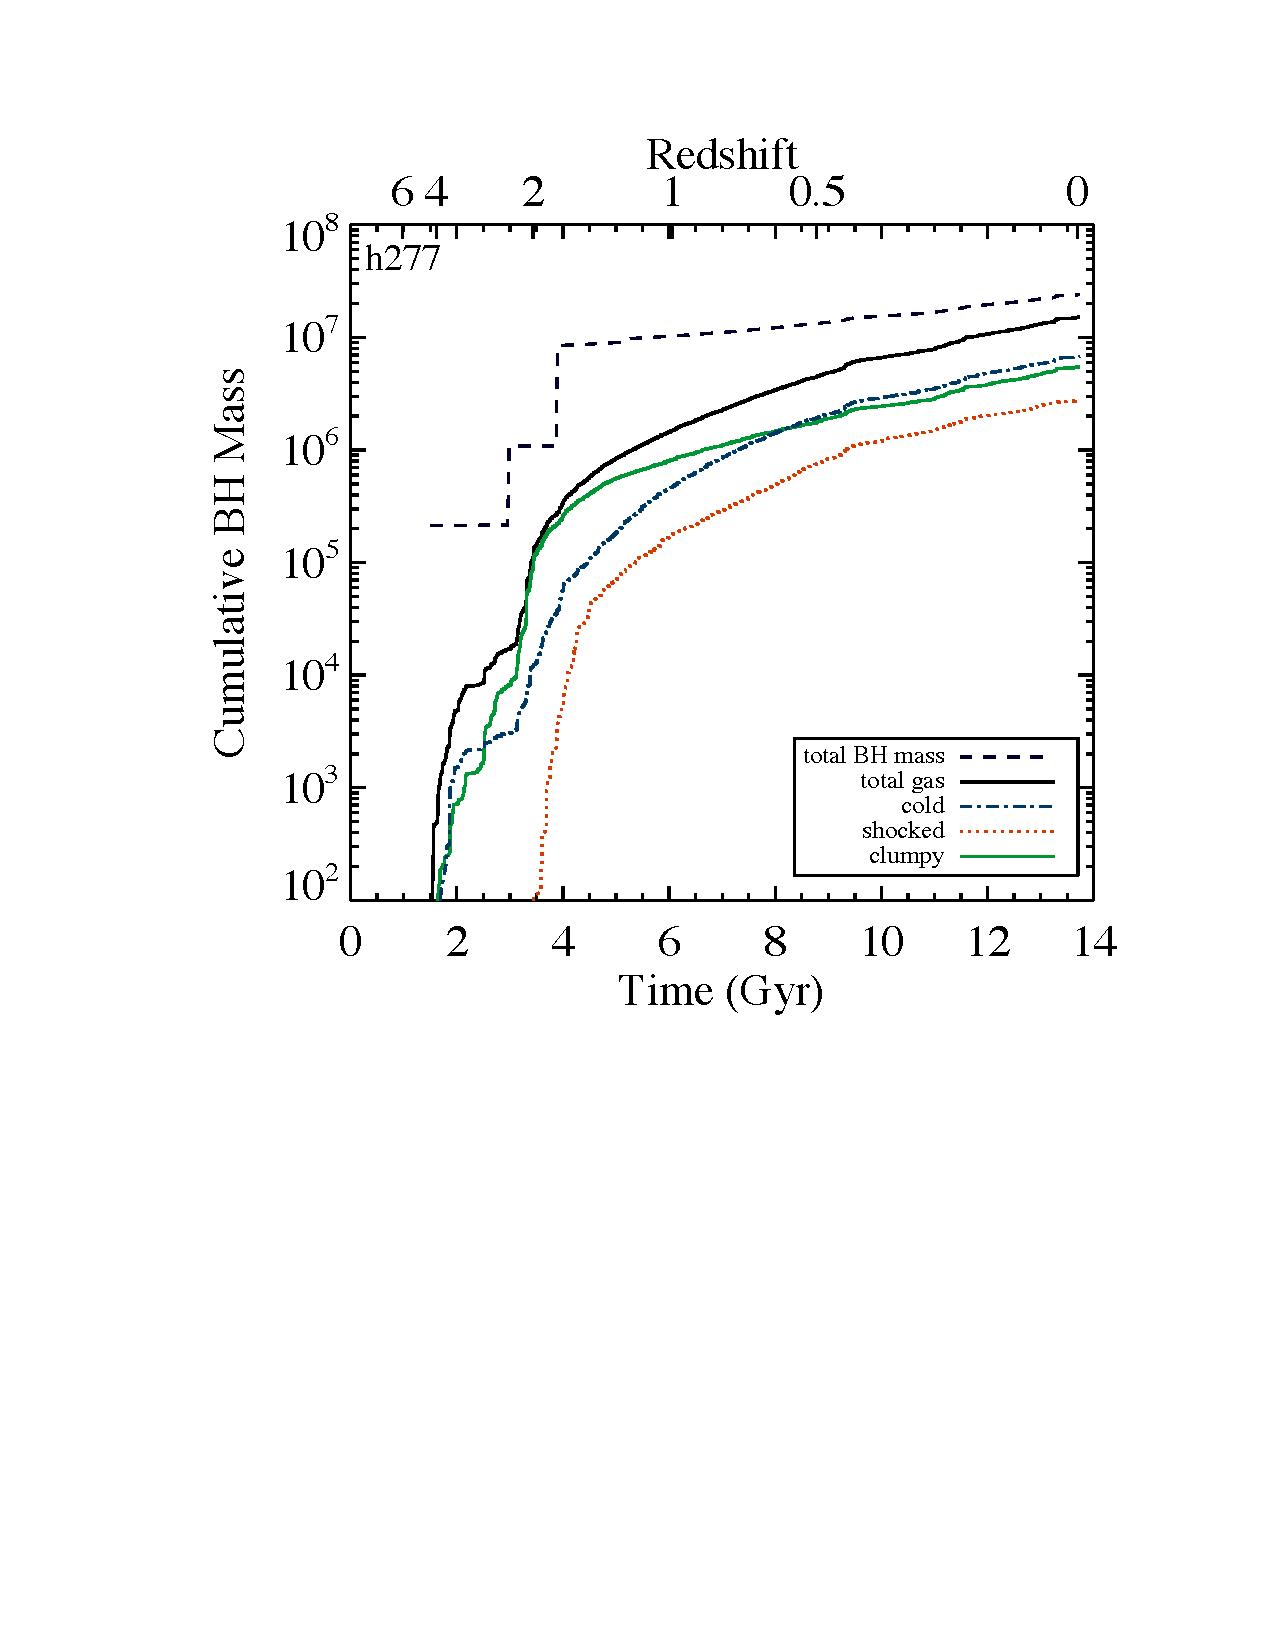
\includegraphics[angle=0]{h277_allmassgas_final}}}
\caption[]{The central BH’s cumulative mass as a function of time and redshift. The black dashed line indicates the total cumulative BH mass. The black solid line indicates the total gas mass. The blue dot-dashed line indicates the gas mass accreted via unshocked gas. The green solid line indicates the gas mass accreted through mergers. The red dashed line indicates gas mass that was shocked upon entry into the halo.}
\label{h277allmassgas} 
\end{figure}

\begin{figure}
\centerline{\resizebox{0.75\hsize}{!}{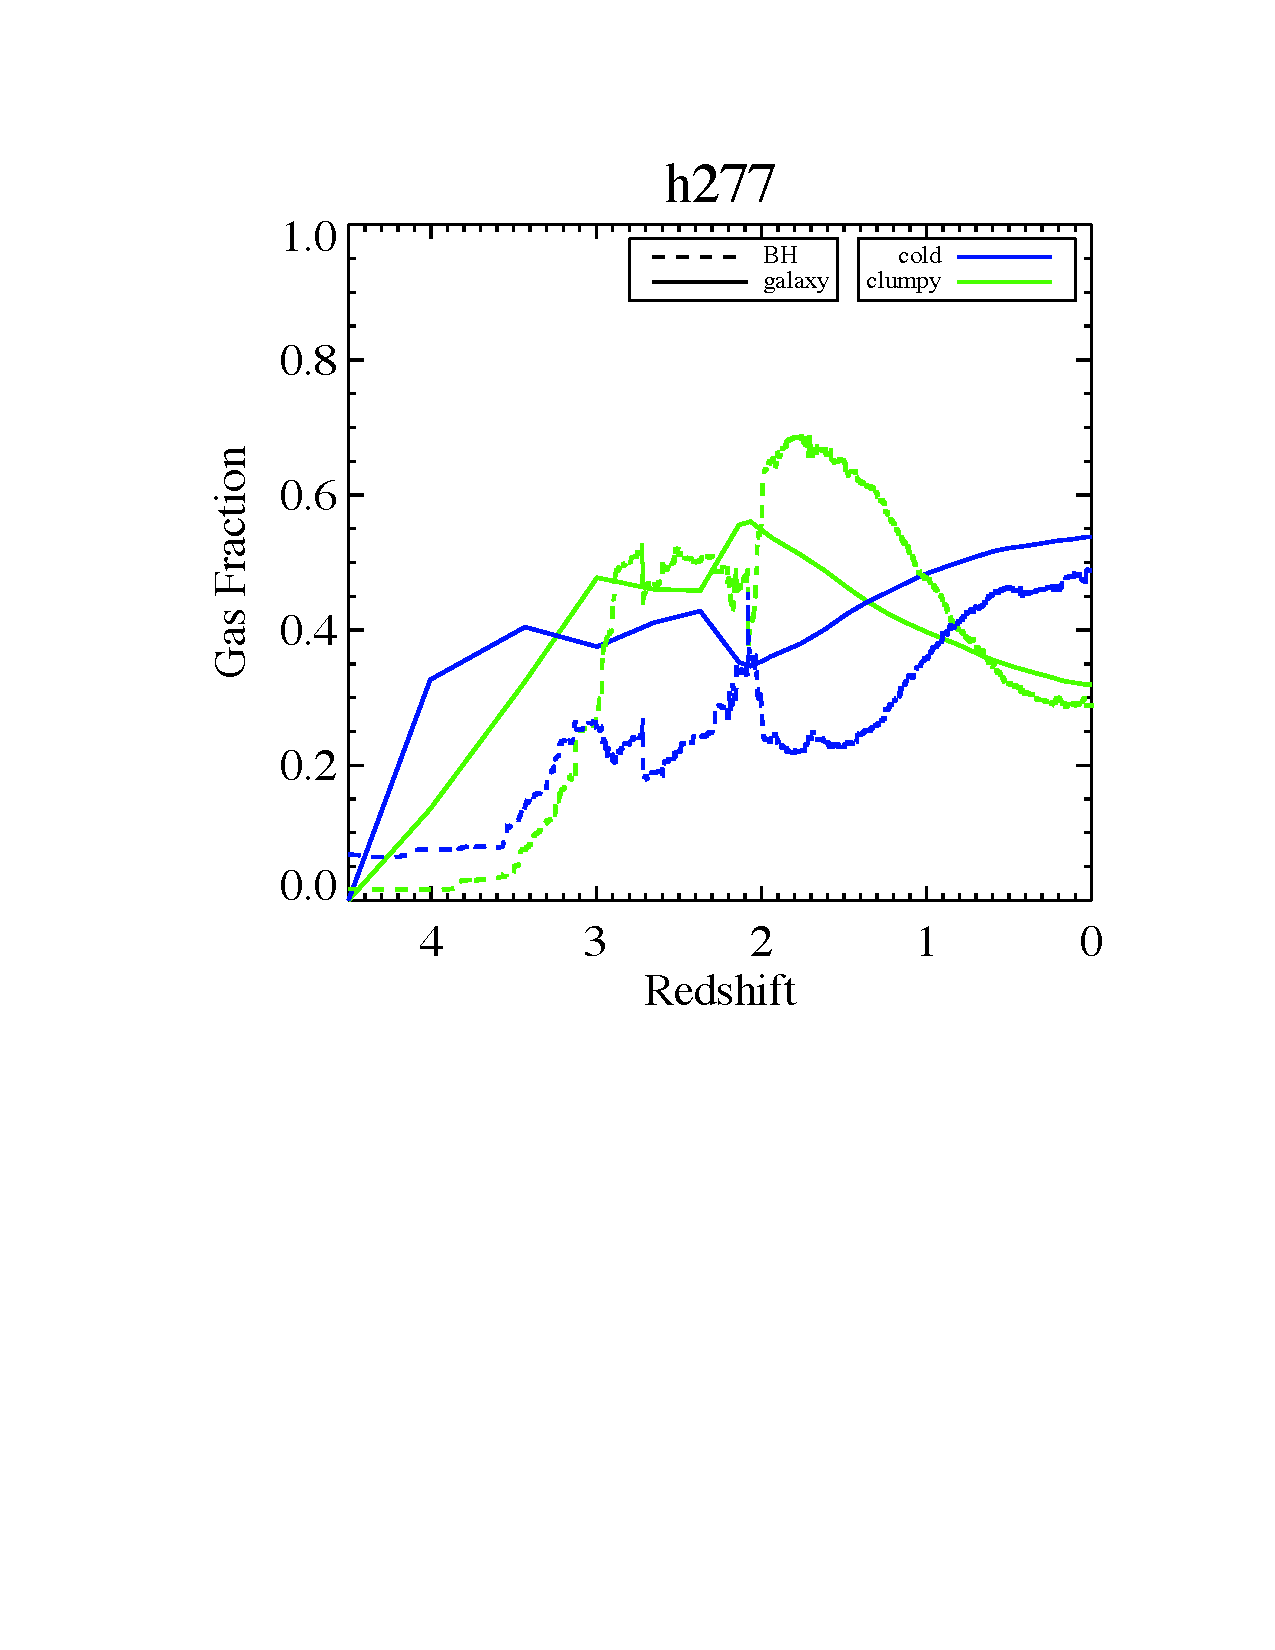
\includegraphics[angle=0]{h277numfraction_brightgreen}}}
\caption[]{Gas fraction across redshift for galaxy (solid lines) and central BH (dashed lines). Green lines signify gas fractions accreted via mergers and blue lines designate gas accreted via unshocked gas filaments.}
\label{h277numfrac} 
\end{figure}

\begin{figure}
\centerline{\resizebox{0.75\hsize}{!}{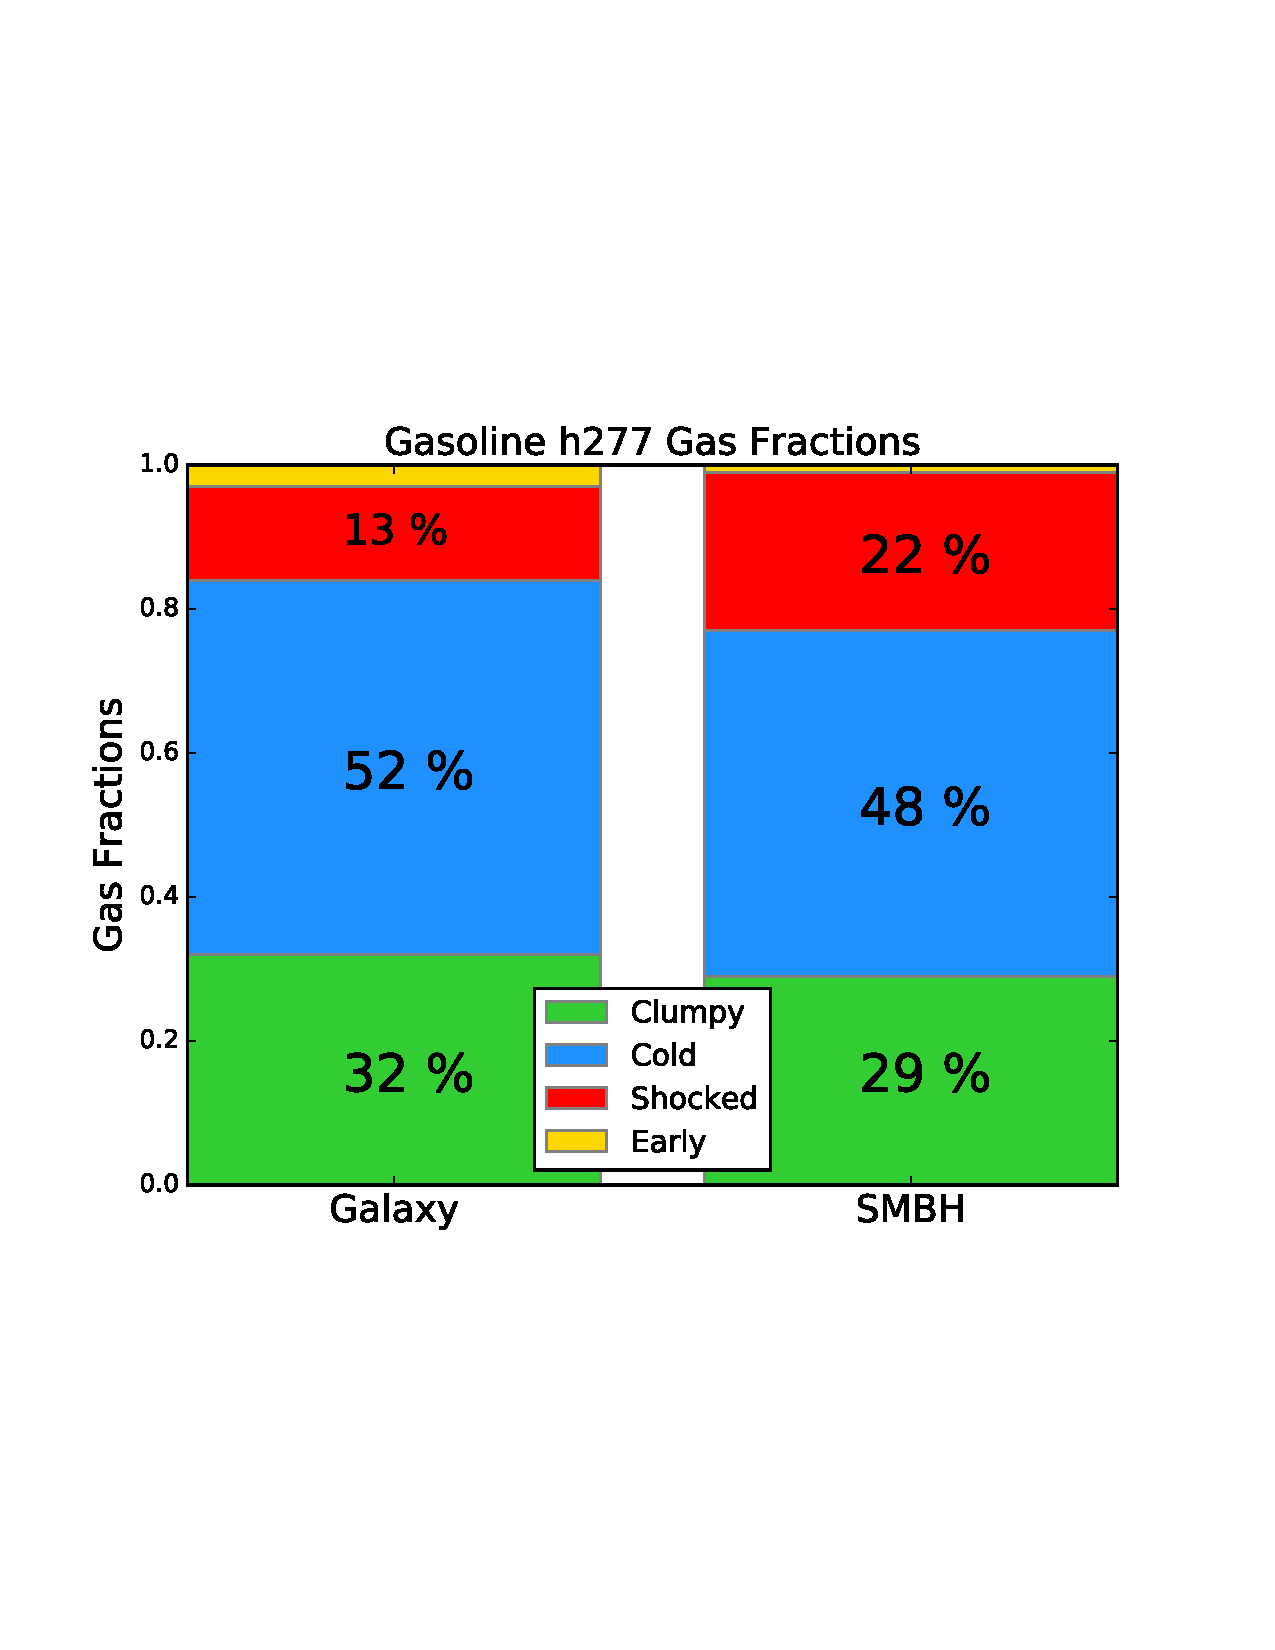
\includegraphics[angle=0]{h277_stackbarfractions}}}
\caption[]{Gas fractions of the gas particles accreted in h258 by the main halo (left) and the SMBH (right), distinguished by type. Blue, green, and red distinguish gas gained through unshocked gas, gained through mergers, and gas shocked upon entry, respectively. Yellow indicates gas that existed within the main halo upon formation; this ``early'' gas is negligable ($<$ 1 \%) within the SMBH.}
\label{h277stackfrac} 
\end{figure}

\begin{figure}
\centerline{\resizebox{0.75\hsize}{!}{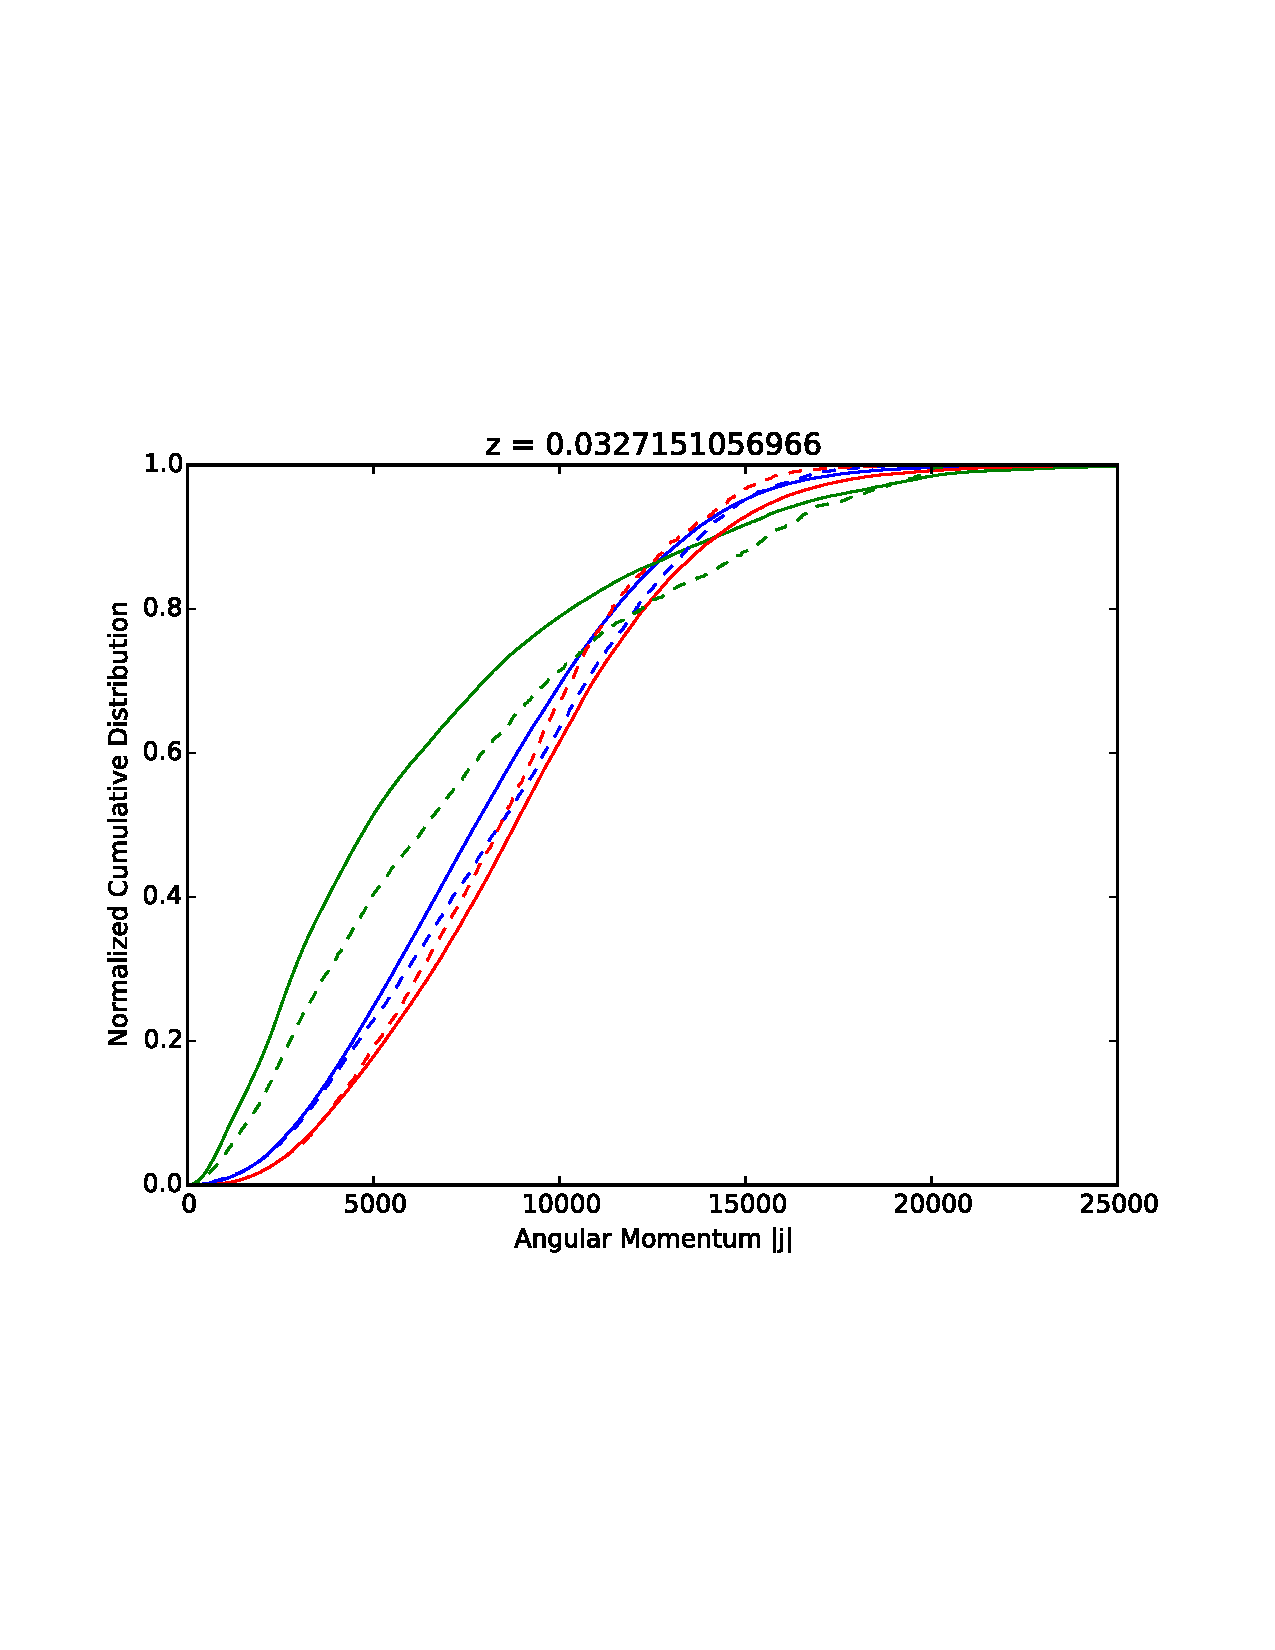
\includegraphics[angle=0]{h277_angmom_cumudist}}}
\caption[]{ Cumulative distribution of angular momentum of the gas particles accreted onto h277.  Gas particles accreted onto the main halo (solid lines) and central black hole (dashed lines). The green, blue, and red lines indicate clumpy, unshocked, and shocked gas, respectively.}
\label{h277angmom} 
\end{figure}

\begin{figure}
\centerline{\resizebox{0.75\hsize}{!}{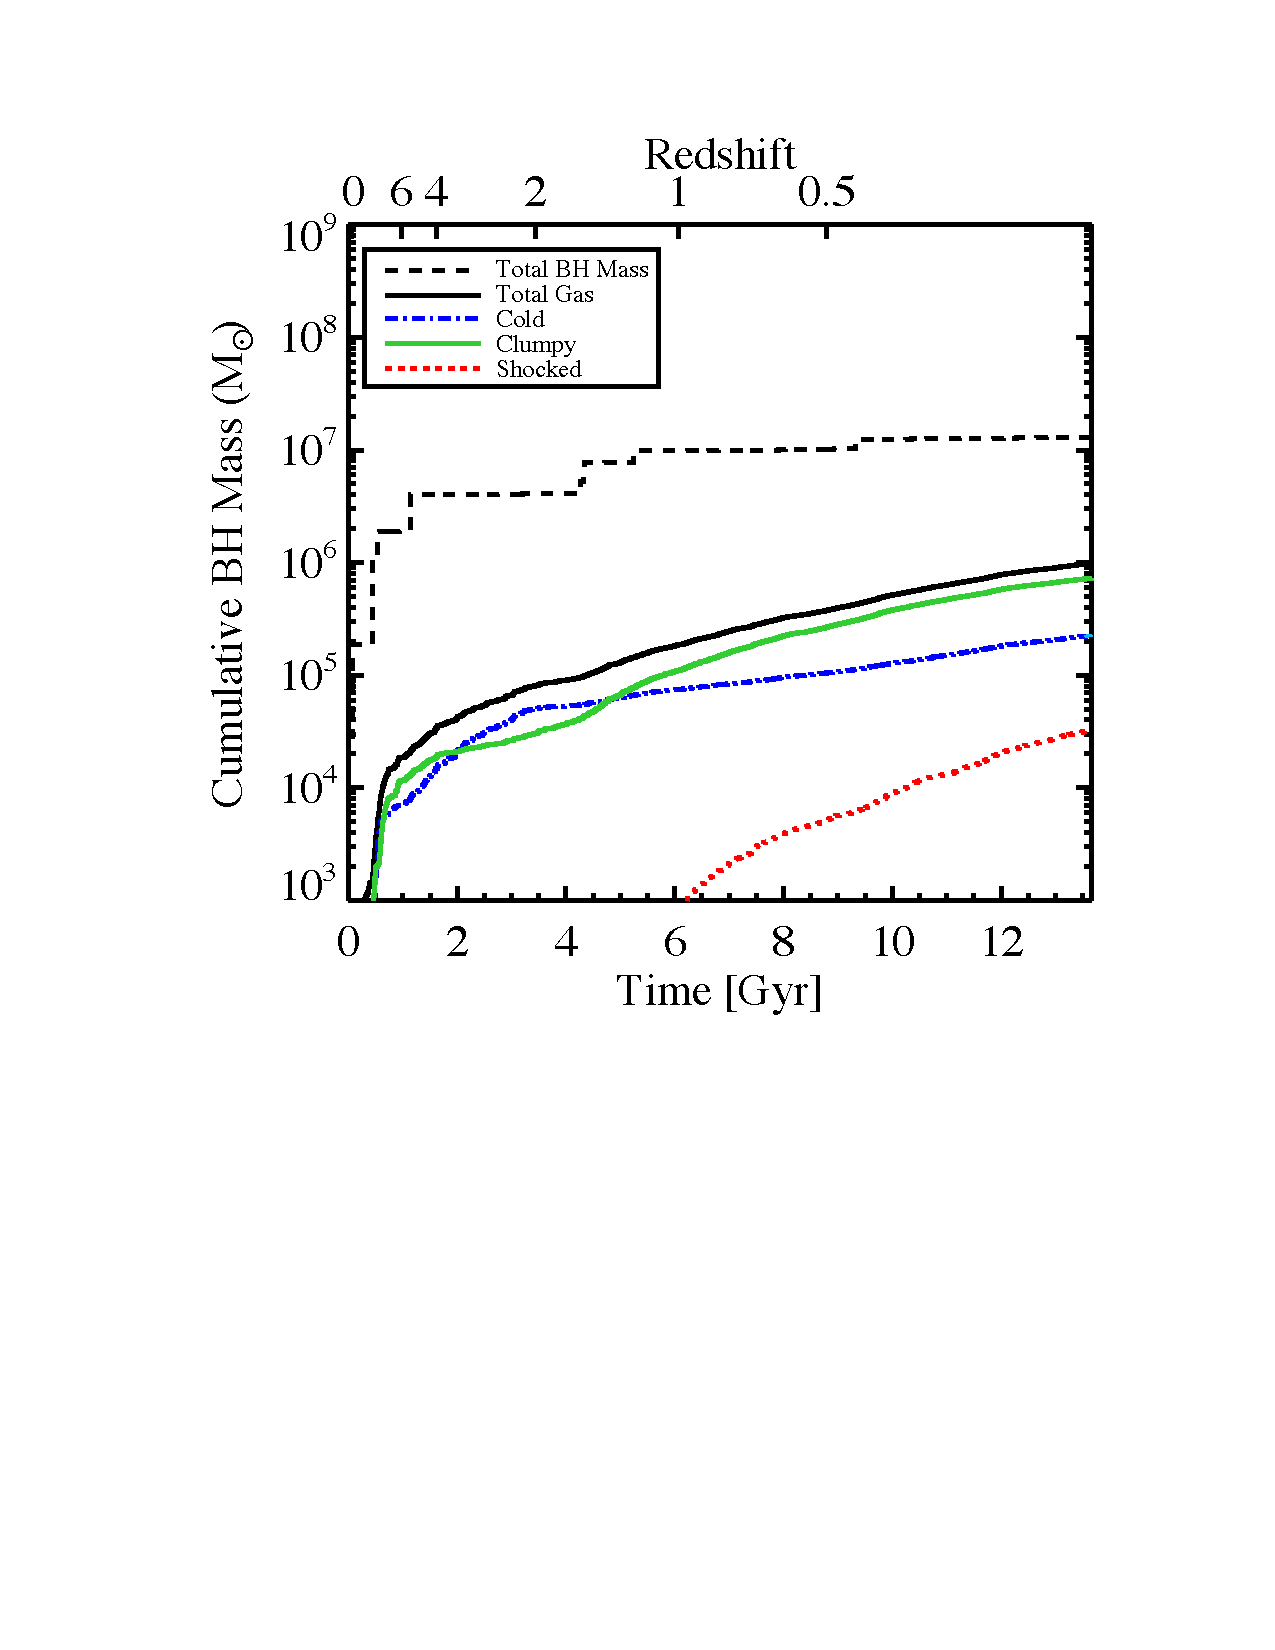
\includegraphics[angle=0]{hrh258_massgastime}}}
\caption[]{The central BH’s cumulative mass as a function of time and redshift. The black dashed line indicates the total cumulative BH mass. The black solid line indicates the total gas mass. The blue dot-dashed line indicates the gas mass accreted via unshocked gas. The green solid line indicates the gas mass accreted through mergers. The red dashed line indicates gas mass that was shocked upon entry into the halo.}
\label{hrh258allmassgas} 
\end{figure}

\begin{figure}
\centerline{\resizebox{0.75\hsize}{!}{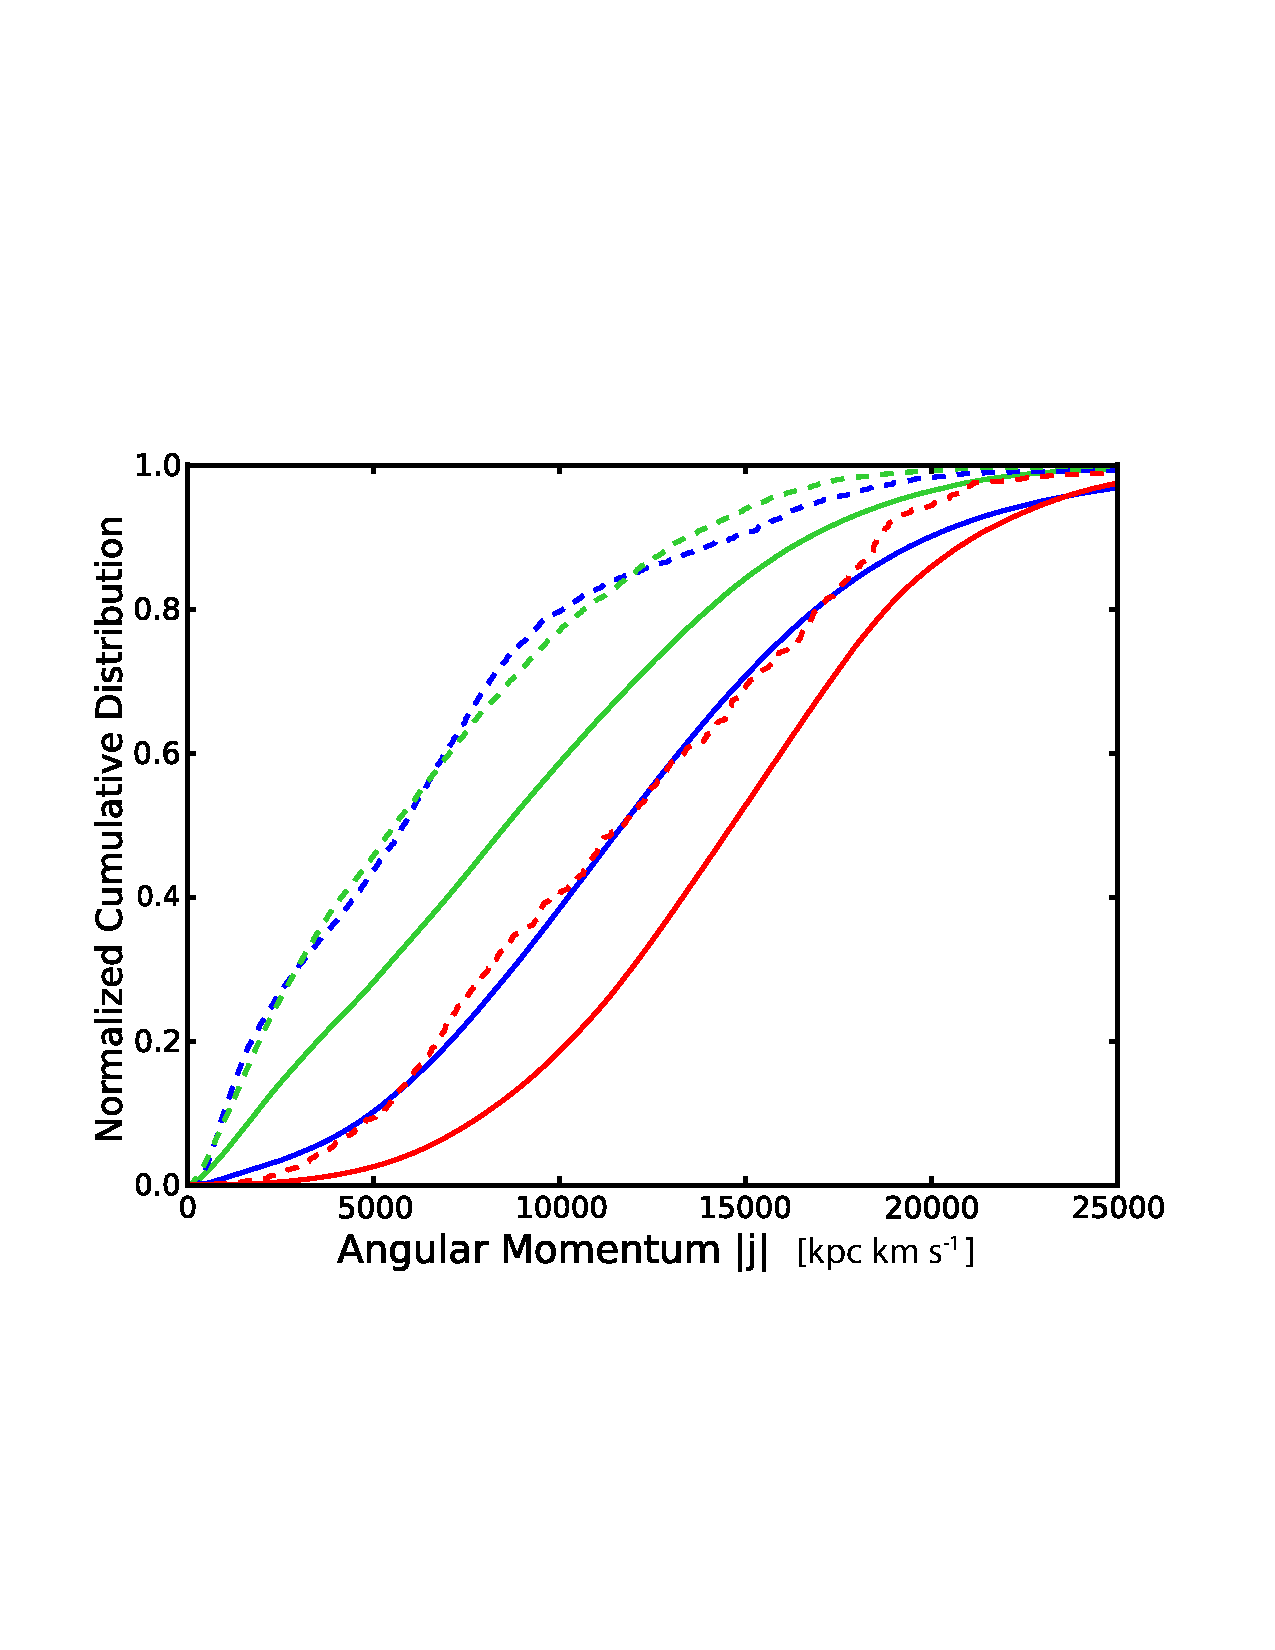
\includegraphics[angle=0]{hrh258_am_cumu_4096}}}
\caption[]{ Cumulative distribution of angular momentum of the gas particles accreted onto the high resolution ChaNGa h258.  Gas particles accreted onto the main halo (solid lines) and central black hole (dashed lines). The green, blue, and red lines indicate clumpy, unshocked, and shocked gas, respectively.}
\label{hrh258angmom} 
\end{figure}

\begin{figure}
\centerline{\resizebox{0.75\hsize}{!}{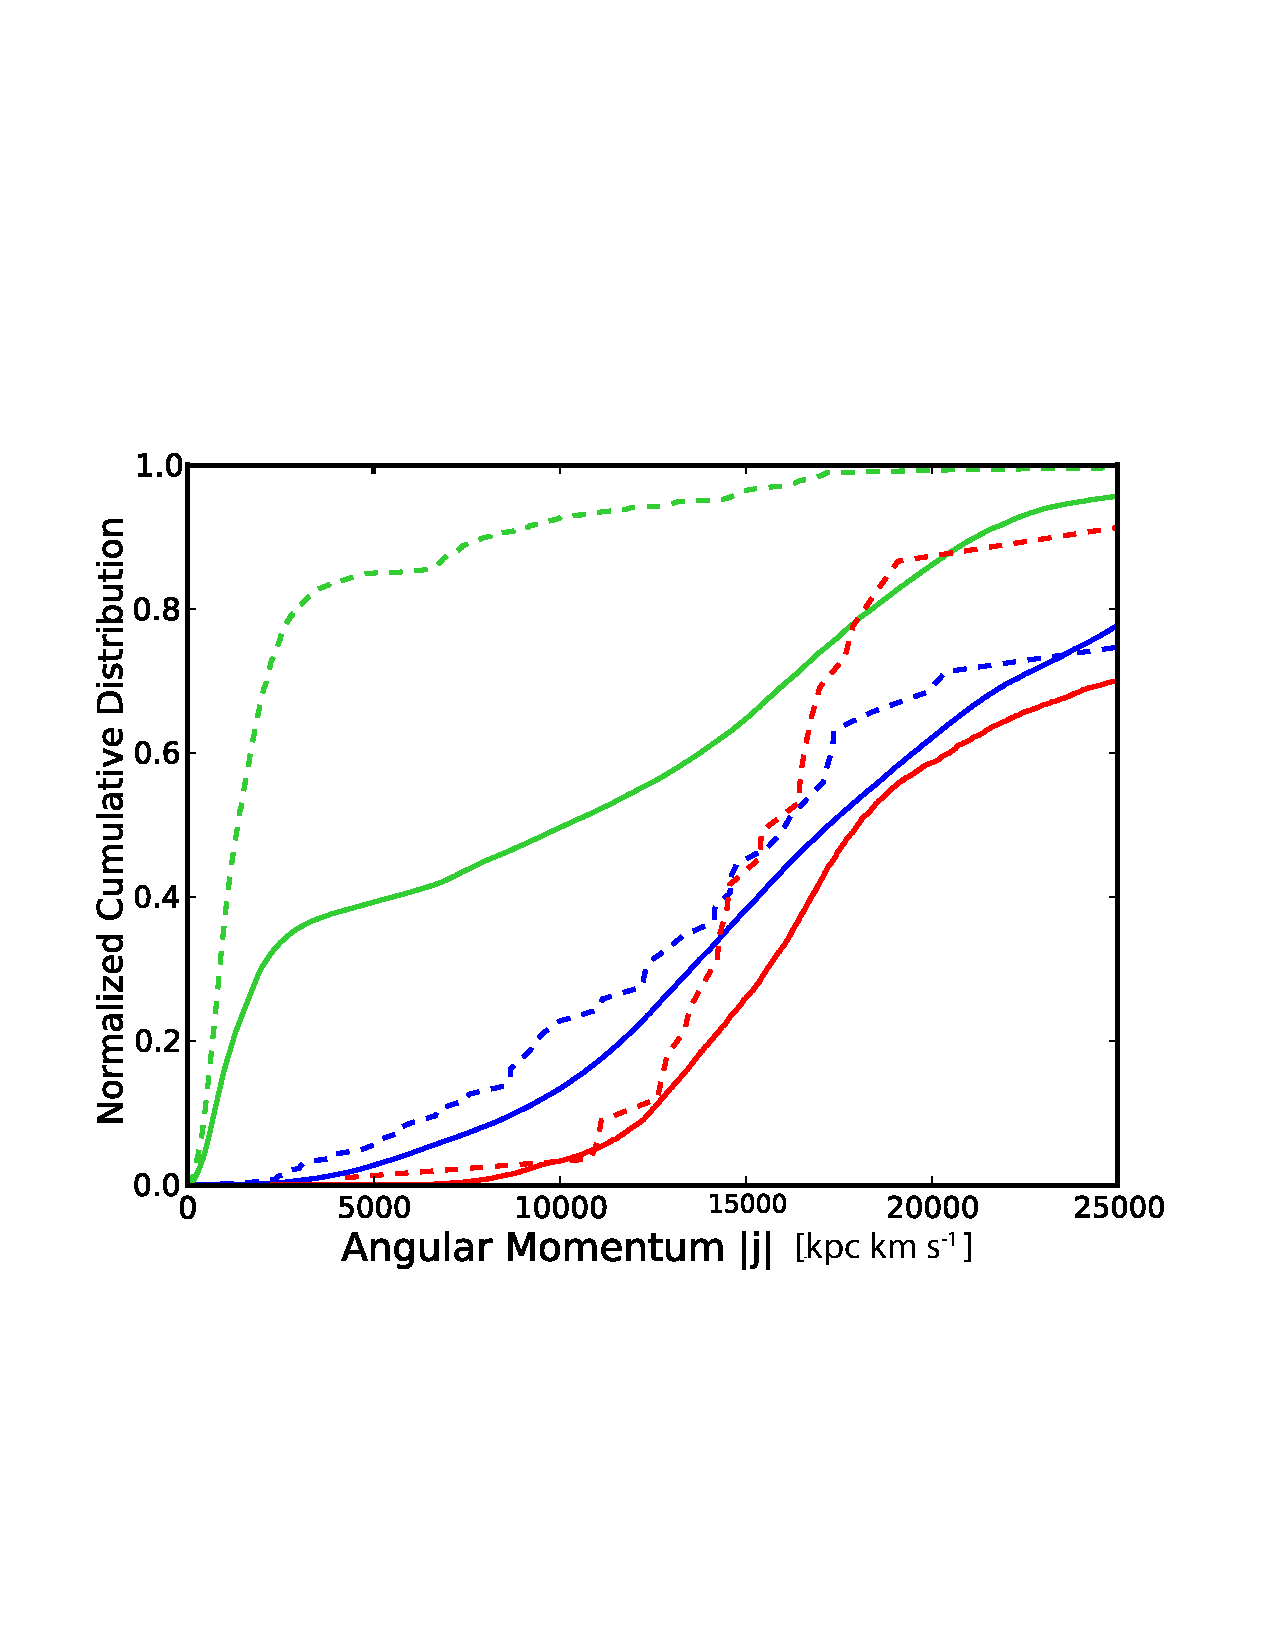
\includegraphics[angle=0]{hrh258_am_tsnew_1584}}}
\caption[]{ Cumulative distribution of angular momentum of the gas particles accreted onto the high resolution ChaNGA h258 galaxy at the time of the major merger (z ~ 1). There are about 450,000 gas particles accreted at this timestep, which gas particles accreted onto the main halo and central black hole distinguished by solid and dashed lines. The green, blue, and red lines indicate clumpy, unshocked, and shocked gas, respectively.}
\label{hrh258angmom_merger} 
\end{figure}

\begin{figure}
\centerline{\resizebox{0.75\hsize}{!}{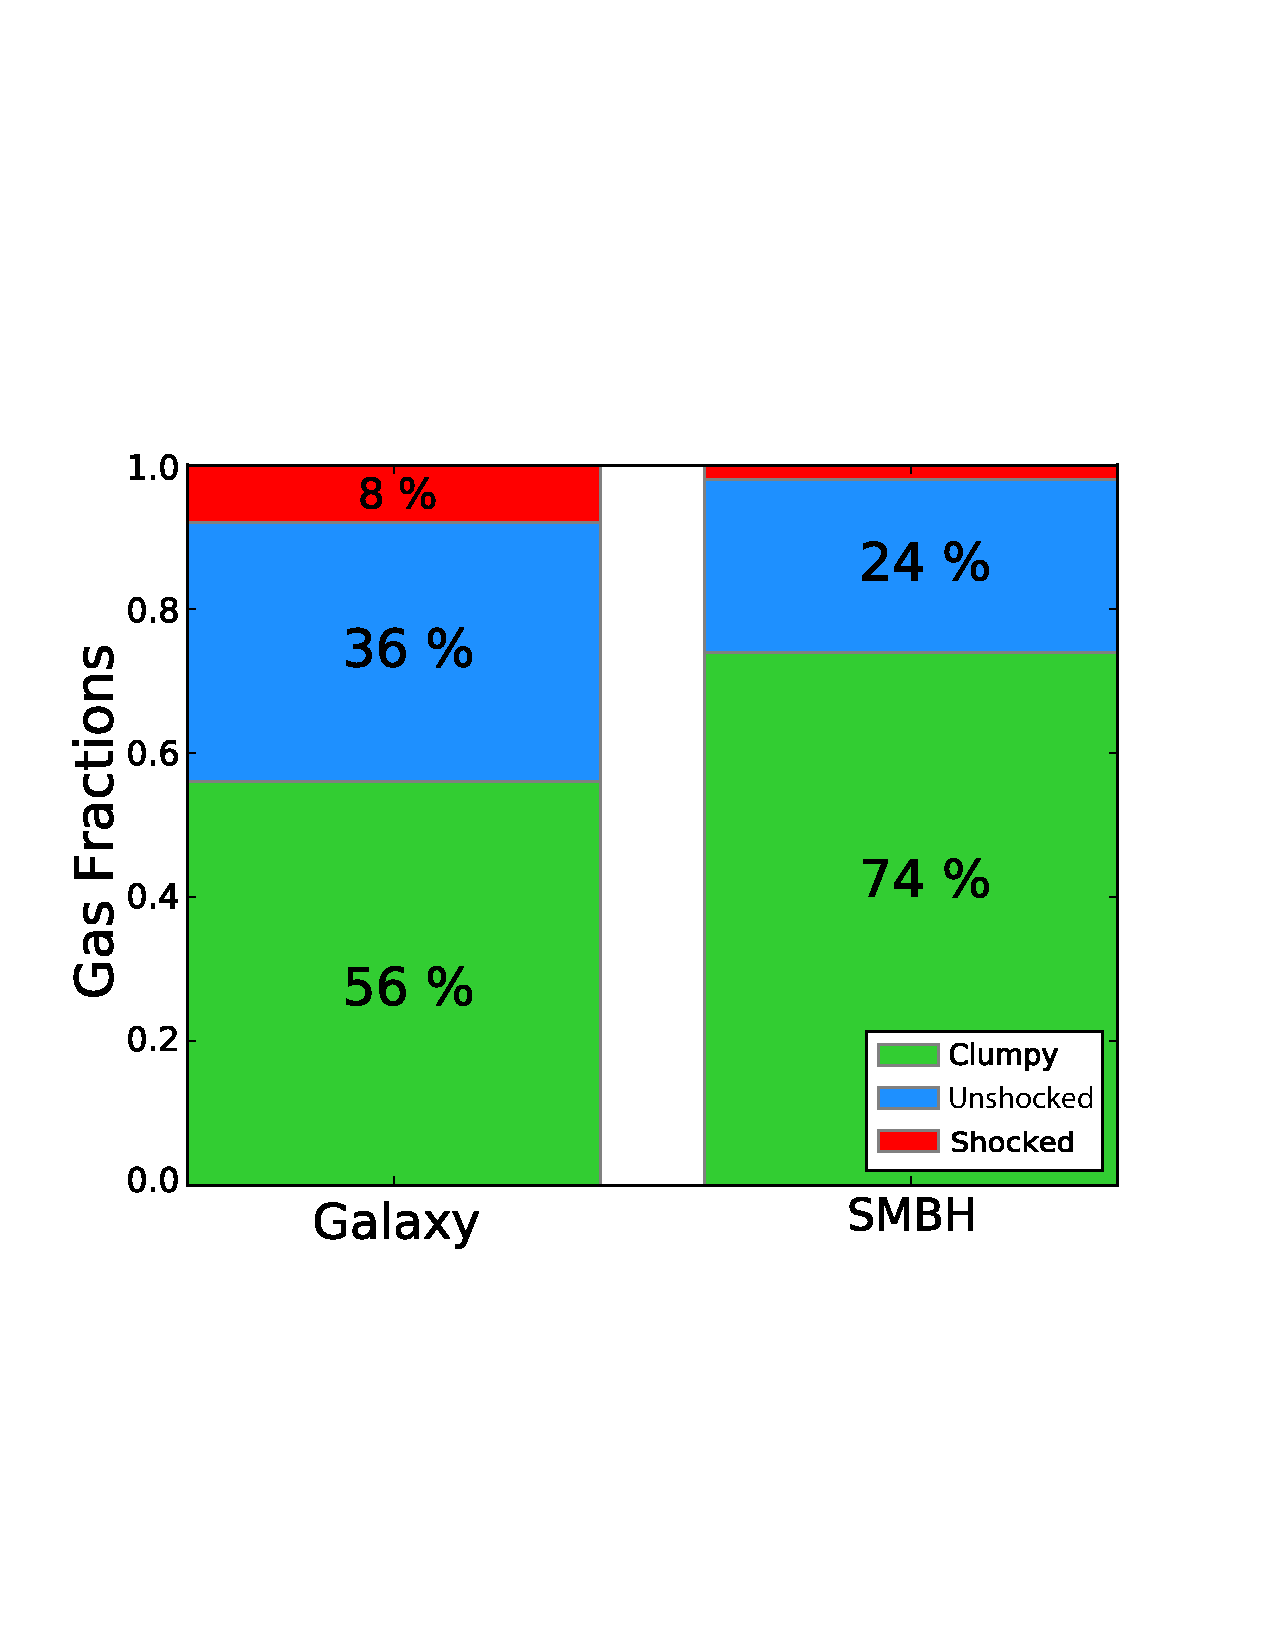
\includegraphics[angle=0]{hrh258_stackbarfractions}}}
\caption[]{Gas fractions of the gas particles accreted by the high resolution ChaNGA h258 by the main halo (left) and the SMBH (right), distinguished by type. Blue, green, and red distinguish gas gained through unshocked gas, gained through mergers, and gas shocked upon entry, respectively. Yellow indicates gas that existed within the main halo upon formation; this ``early'' gas is negligable ($<$ 1 \%) within the SMBH.}
\label{h277stackfrac} 
\end{figure}


\bibliography{/Users/nicolesanchez/Documents/MENDELEY/MEND_bibtexfiles/Sanchez2016.bib}


\end{document}

